


\documentclass[review,authoryear,3p]{elsarticle}

\usepackage{amsmath}
\usepackage{amssymb}
\usepackage{graphicx}
\usepackage{setspace} 
\usepackage[usenames,dvipsnames]{color}

% \newcommand{\dean}[1]{\textsf{\emph{\textbf{\textcolor{red}{#1}}}}}
\newcommand{\dean}[1]{\textcolor{red}{#1}}
\newcommand{\parham}[1]{\textcolor{blue}{#1}}
\newcommand{\mike}[1]{\textcolor{Plum}{#1}}

\journal{Neuroimage}
\begin{document}
\begin{frontmatter}
\title{A Data-Driven Framework for Neural Field Modeling}

\author[DEEE,BEI,UE]{D. R. Freestone \corref{cor1} \fnref{fn1}}
\ead{dfreestone@bionicear.org}
\author[US]{P. Aram\fnref{fn1}} 
\ead{p.aram@sheffield.ac.uk}
\author[UE,CU]{M. Dewar}
\ead{mike.dewar@columbia.edu}
\author[UM]{K. Scerri}
\ead{kenneth.scerri@um.edu.mt}
\author[DEEE,BEI]{D. B. Grayden}
\ead{grayden@unimelb.edu.au}
\author[US]{V. Kadirkamanathan}
\ead{visakan@sheffield.ac.uk}

\address[DEEE]{Department of Electrical and Electronic Engineering, University of Melbourne, Melbourne, VIC, Australia}
\address[BEI]{The Bionic Ear Institute, East Melbourne, VIC, Australia}
\address[UE]{Institute for Adaptive and Neural Computation, University of Edinburgh, Edinburgh, UK}
\address[US]{Department of Automatic Control and Systems Engineering, University of Sheffield, Sheffield, UK}
\address[CU]{Department of Applied Physics and Applied Mathematics, Columbia University, New York, NY, USA}
\address[UM]{Department of Systems and Control Engineering, University of Malta, Msida, MSD, Malta}

\fntext[fn1]{Authors contributed equally to this work.}
\cortext[cor1]{Corresponding author}

\begin{abstract}
This paper presents a framework for creating neural field models from electrophysiological data. The Wilson and Cowan or Amari style neural field equations are used to form a parametric model, where the parameters are estimated from data. To illustrate the estimation framework, data is generated using the neural field equations incorporating modeled sensors enabling a comparison between the estimated and true parameters. To facilitate state and parameter estimation, we introduce a method to reduce the continuum neural field model using a basis function decomposition to form a finite-dimensional state-space model. Spatial frequency analysis methods are introduced that systematically specify the basis function configuration required to capture the dominant characteristics of the neural field. The estimation procedure consists of a two-stage iterative algorithm incorporating the unscented Rauch-Tung-Striebel smoother for state estimation and a least squares algorithm for parameter estimation. The results show that it is theoretically possible to reconstruct the neural field and estimate intracortical connectivity structure and synaptic dynamics with the proposed framework. 
\end{abstract}

\begin{keyword}
	Neural Field Model \sep Nonlinear Estimation \sep Intracortical Connectivity \sep Nonlinear Dynamics
\end{keyword}

\end{frontmatter}

\section{Introduction}

Generating physiologically plausible neural field models is of great importance for studying brain dynamics at the mesoscopic and macroscopic scales. While our understanding of the function of neurons is well developed, the overall behaviour of the brain's mesoscopic and macroscopic scale dynamics remains largely theoretical. Understanding the brain at this level is extremely important since it is at this scale that pathologies such as epilepsy, Parkinson's disease and schizophrenia are manifested. 

Mathematical neural field models provide insights into the underlying physics and dynamics of electroencephalography (EEG) and magnetoencephalography (MEG) (see~\citet{Deco2008,David2003} for recent reviews). These models have demonstrated possible mechanisms for the genesis of neural rhythms (such as the alpha and gamma rhythms) \citep{Liley1999,RENNIE2000}, epileptic seizure generation \citep{DaSilva2003,Suffczynski2004,Wendling2005} and insights into other pathologies \citep{Moran2008,Schiff2009} that would be difficult to gain from experimental data alone. 

Unfortunately, the use of these models in the clinic has been limited, since they are constructed for ``general'' brain dynamics whereas pathologies almost always have unique underlying patient-specific causes. Patient-specific data from electrophysiological recordings is readily available in the clinical setting, particularly from epilepsy surgery patients, suggesting an opportunity to make the patient-specific link to models of cortical dynamics. Furthermore, recent technological advances have driven an increased level of sophistication in recording techniques, with dramatic increases in spatial and temporal sampling \citep{Brinkmann2009}. However, the mesoscopic and macroscopic neural dynamic state is not directly observable in neurophysiological data, making predictions of the underlying physiology inherently difficult.

For models to be clinically viable, they must be patient-specific. A possible approach to achieve this would be to fit a general continuum neural field model, like the \citet{Wilson1973} (WC) or \citet{Amari1977} models, or a neural mass model like the \citet{Jansen1995} model, to patient-specific data. Fitting the neural models to individuals is a highly non-trivial task. Recently, however, this task has been approached from a number of standpoints. \dean{(Reviewer 1, additional comment d):) The first paper on patient-specific modeling came from~\citet{Valdes1999}, where they fit the neural mass model of \citet{LopesDaSilva1976} and \citet{Zetterberg1978} to EEG data using the local linearization filter \citep{Ozaki1993,Ozaki1994,Ozaki2000}. This paper demonstrated for the first time the feasibility of assimilating data with neural models of EEG.} 

Perhaps the most accepted estimation framework for neural mass models is dynamical causal modeling (DCM) \citep{David2003,David2006}, which has been proposed for studying evoked potential dynamics. This framework can be viewed as an extension to the work of~\citet{Valdes1999} allowing for coupling of neural masses. Via a Bayesian inference scheme, DCM estimates the long range (cortico-cortical) connectivity structure between the specific isolated brain regions that best explains a given data set using the model of \citet{Jansen1995}.

\dean{(Reviewer 1, additional comment d):) Data-driven neural modeling was extended to the continuum approximation by \citet{Galka2008}, where they proposed an estimation framework based on a linear damped wave equation. Using a Kalman filter maximum likelihood framework, they improved on the low resolution electromagnetic tomography (LORETA) method for solving the inverse EEG problem. Another continuum neural field model-based estimator was developed by \citet{Daunizeau2009}, as an extension to the DCM framework. \parham{They argue that using a spatially extended continuum field model is superior for explaining cortical function than the neural mass DCM, since field models can explain a richer repertoire of dynamics such as traveling waves and bump solutions.}}   

\dean{Another recent approach estimates the parameters of a modified WC neural field model using an unscented Kalman filter~\citep{schiff2008kalman}. This work takes a systems theoretic approach to the neural estimation problem, successfully demonstrating that it is possible to perform state estimation and control on spatiotemporal neural fields. This marks the first step in what has the potential to revolutionize the treatment of many neurological diseases where therapeutic electrical stimulation is viable. For other valuable contributions to data-driven neural modeling, see \citet{Nunez2000}, \citet{Jirsa2002}, and \citet{Robinson2004}.}

We present an extension to the work of \citet{schiff2008kalman} by establishing a framework for estimating the state of the WC equations for larger scale (more space) systems via a systematic model reduction procedure. In addition, a new method is presented for estimating the connectivity structure and the synaptic dynamics. Until now, model-based estimation of local intracortical connectivity has not been reported in the literature (to the best of the authors' knowledge). Our study also extends recent work which shows that it is possible to estimate local coupling of spatiotemporal systems using techniques from control systems theory and machine learning \citep{Dewar2009}. The key development of this previous work was to represent a spatiotemporal system as a standard state-space model, with the number of states independent of the number of observations (recording electrodes in this case). In addition, the appropriate model selection tools have been developed \citep{Scerri2009} allowing for the application of the technique to neural fields. This paper extends the linear framework of \citet{Dewar2009} and \citet{Scerri2009} to the nonlinear case required for the neural field equations. 

Modeling the neural dynamics within this framework has a distinct advantage over the more standard multivariate auto-regressive (MVAR) models: the number of parameters to define the spatial connectivity is considerably smaller than the number of AR coefficients typically required to achieve the model complexity. 

In this paper, we demonstrate for the first time how an intracortical connectivity kernel can be inferred from data, based on a variant of the \citet{Wilson1973} neural field model. This work provides a fundamental link between the theoretical advances in neural field modeling and \dean{(for reviewer 1, comment 3:) high resolution intracranial} electrophysiological data. \dean{(for reviewer 1 comment 1:) (this is copied from the abstract) To illustrate the estimation framework, data is generated using the neural field equations incorporating modeled sensors enabling a comparison to be made between the estimated and true parameters.} The paper proceeds by first describing the continuum neural field equations that are used as the cortical model. Then a finite-dimensional neural field model is derived. The model is reduced by approximating the neural field using a set of continuous basis functions, weighted by a finite dimensional state vector. The next section establishes conditions, using spatial frequency analysis, for both sensor and basis function spacing and width, such that the dominant dynamics of the neural field can be represented by the reduced model. The state and parameter estimation procedure is described in the following section. The results for the spatial frequency analysis and parameter estimation are then presented. Finally, the implications and limitations of this framework are discussed along with planned future developments.

\section{Methods}

\subsection{Neural Field Model}\label{NeuralModelSection} 
Neural field models relate mean firing rates of pre-synaptic neural populations to mean post-synaptic membrane potentials. They are popular as they are parsimonious yet have a strong link with the underlying physiology. Each neural population represents a functional cortical processing unit, such as a column. The columnar organization of the cortex is continuous, where pyramidal cells are members of many columns. In general, cortical structure can be modeled in a physiologically plausible manner as being locally homogeneous (in short range intracortical connectivity) and heterogeneous (in long range cortico-cortical and corticothalamic connectivity) \citep{Jirsa2009,Qubbaj2007}. In certain regions of the cortex, each column is thought to be connected locally via symmetric short range local excitation with surround inhibition \citep{Braitenberg1998}. For example, this structural organization is most studied in the visual system, where the surrounding inhibition effectively tunes a cortical column to a particular receptive visual field \citep{Sullivan2006}. Neural field models are descriptive of a range of neurodynamics of the cortex such as evoked potentials, visual hallucinations and epileptic behaviour \citep{David2003,Bressloff2001,Breakspear2006}. Field models are also capable of generating complex spatial patterns of activity such as Turing patterns, spirals and traveling oscillations \citep{Amari1977,Coombes2005,Coombes2007}.

\subsection{Integro-Difference Equation Neural Field Model}\label{IntegroDifferenceEquationSection} 
The combination of modeling techniques in this paper leads to a large amount of notation, so a reference of the symbols used is provided in Table~\ref{tab:Notation}. The model relates the average number of action potentials $g(\mathbf{r},t)$ arriving at time $t$ and position $\mathbf{r}$ to the local post-synaptic membrane voltage $v(\mathbf{r},t)$. The post-synaptic potentials generated at a neuronal population at location $\mathbf{r}$ by action potentials arriving from all other connected populations is described by 
\begin{equation}
	\label{SpikesToPotential} v\left( {\mathbf{r},t} \right) = \int_{ - \infty }^t {h\left( {t - t'} \right)g\left( {\mathbf{r},t'} \right) \, dt'}. 
\end{equation}
The post-synaptic response kernel $h(t)$ is described by 
\begin{equation}
	\label{SynapticRespKernel} h(t) = \eta(t)\exp{\left(-\zeta t\right)}, 
\end{equation}
where $\zeta=\tau^{-1}$, $\tau$ is the synaptic time constant and $\eta(t)$ is the Heaviside step function. Non-local interactions between cortical populations at positions $\mathbf{r}$ and $\mathbf{r}'$ are described by 
\begin{equation}
	\label{RateBasedInteractions} g\left( \mathbf{r},t \right) = \int_\Omega {w\left( \mathbf{r},\mathbf{r}' \right)f\left( v\left( \mathbf{r}',t \right) \right)\, d\mathbf{r}'}, 
\end{equation}
where $f(\cdot)$ is the firing rate function, $w(\cdot)$ is the spatial connectivity kernel and $\Omega$ is the spatial domain representing a cortical sheet or surface. The connectivity kernel is typically a ``Mexican hat'' or ``wizard hat'' function, which describes local excitation and surround inhibition. An example of the Mexican hat connectivity kernel used in this paper is shown in Fig.~\ref{fig:Figure1}. To demonstrate flexibility in the estimation algorithm and to model larger cortical regions, a third component of the kernel is introduced describing weak longer-range excitation. The exact shape of this kernel is assumed to vary across subjects, and hence needs to be inferred from subject-specific data.

The firing rate of the presynaptic neurons is related to the post-synaptic membrane potential by the sigmoidal activation function 
\begin{equation}
	\label{ActivationFunction} f\left( v\left( \mathbf{r}', t \right) \right) = \frac{1}{1 + \exp \left( \varsigma \left( v_0 - v\left(\mathbf{r}',t\right) \right) \right)}. 
\end{equation}
The parameter $v_0$ describes the firing threshold of the neural populations and $\varsigma$ governs the slope of the sigmoid. By substituting equation~\ref{RateBasedInteractions} into equation~\ref{SpikesToPotential} we get the spatiotemporal model 
\begin{equation}
	\label{FullDoubleIntModel} v\left(\mathbf{r},t\right) =
	\int_{-\infty}^t 
	h\left(t - t'\right) \int_\Omega
	w\left(\mathbf{r},\mathbf{r}'\right) 
	f\left( v\left( \mathbf{r}',t' \right)\right)
	\, d\mathbf{r}'dt'.
\end{equation}
\parham{The post-synaptic membrane potential is in fact the temporal convolution between the synaptic kernel and the average firing rate
\begin{equation}\label{FullConvolutionModel}
 v\left(\mathbf r,t\right)= \left(h\ast g\right)\left(\mathbf r,t\right)
\end{equation}
where $\ast$ denotes the convolution operator.}
\dean{(reviewer 2, comment 3:) \parham{To obtain (To arrive at)} the standard integro-differential equation form of the model, we use the fact that the synaptic response kernel is a Green's function of a linear differential equation defined by the differential operator $\textrm{D}=d/dt + \zeta$. A Green's function satisfies
\begin{equation}
	\label{GreensFuncDef} \textrm{D}h\left( t \right) = \delta \left( t \right), 
\end{equation} 
where $\delta(t)$ is the Dirac-delta function. Applying the differential operator $\textrm{D}$ \parham{to equation~\ref{FullConvolutionModel}} gives
\begin{align}
 \textrm{D}v\left(\mathbf r,t\right)&= \textrm{D}\left(h\ast g\right)\left(\mathbf r,t\right)\\
&=\left(\textrm{D}h\ast g\right)\left(\mathbf r,t\right)\\
&=\left(\delta \left(t\right)\ast g\right)\left(\mathbf r,t\right)\\
&=g\left(\mathbf r,t\right)
\end{align}
} This gives the standard form of the model
\begin{equation}
	\label{FinalFormContinuous} 
	\frac{dv\left( \mathbf{r},t \right)}{dt} + \zeta v\left( \mathbf{r},t \right) = \int_\Omega {w\left( \mathbf{r},\mathbf{r}' \right)f\left( {v\left( \mathbf{r}',t \right)} \right)\, d\mathbf{r}'}. 
\end{equation}
To arrive at the integro-difference equation (IDE) form of the model, we discretize time using a first-order Euler method (see \ref{App:Time Discretization} for derivation) giving 
\begin{equation}
	\label{DiscreteTimeModel} 
	v_{t+T_s}\left(\mathbf{r}\right) = 
	\xi v_t\left(\mathbf{r}\right) + 
	T_s \int_\Omega { 
	    w\left(\mathbf{r},\mathbf{r}'\right)
	    f\left(v_t\left(\mathbf{r}'\right)\right) 
	\, d\mathbf{r}'} 
	+ e_t\left(\mathbf{r}\right), 
\end{equation}
where $T_s$ is the time step, $\xi = 1-T_s\zeta $ and $e_t(\mathbf{r})$ is an $i.i.d.$ disturbance such that $e_t(\mathbf{r})\sim\mathcal{GP}(\mathbf 0,\gamma(\mathbf{r}-\mathbf{r}'))$. Here $\mathcal{GP}(\mathbf 0,\gamma(\mathbf{r}-\mathbf{r}'))$ denotes a zero mean Gaussian process with spatial covariance function $\gamma(\mathbf{r}-\mathbf{r}')$ (\cite{Rasmussen2005}). The disturbance is added to account for model uncertainty and unmodeled inputs. To simplify the notation, the index of the future time sample, $t+T_s$, shall be referred to as $t+1$ throughout the rest of the paper. 

The mapping between the membrane voltage and the electrophysiological data, denoted by $\mathbf{y}_t$, is modeled using the observation function that incorporates sensors with a spatial extent by
\begin{equation}\label{eq:ObservationEquation}
	y_t(\mathbf{r}_n) = \int_{\Omega} { m\left(\mathbf{r}_n-\mathbf{r}'\right) v_t\left(\mathbf{r}'\right) \, d\mathbf{r}'} + \varepsilon_t(\mathbf{r}_n), 
\end{equation}
where $m\left(\mathbf{r}_n-\mathbf{r}'\right)$ is the observation kernel, $\mathbf{r}_n$ defines the location of the electrodes in the field, $n=0,...,n_y-1$ indexes the sensors and $\varepsilon_t(\mathbf{r}_n) \sim \mathcal{N}\left(0,\boldsymbol{\Sigma}_{\varepsilon}\right)$ denotes a multivariate normal distribution with mean zero and the covariance matrix $\boldsymbol{\Sigma}_{\varepsilon} = \sigma_{\varepsilon}^2\mathbf{I}$. \dean{(for reviewer 1, comment 3:) Since we are considering intracranial measurements recorded directly from the surface of the cortex or within the brain, the lead field is not modeled by the observation equation.} 

When considering the measurement of a point source in a conductive homogeneous field measured by a point sensor, the observation kernel will theoretically follow a Laplacian like shape, with an exponential decay in the amplitude of a measurement with an increasing distance between the source and sensor \citep{Jackson1999}. However, when considering a source or sensor with a spatial extent, the peak of the observation kernel becomes smoothed and is more similar to a Gaussian shape \citep{Jackson1999}. An experiment supporting this was performed and the results are shown in \ref{App:ObsKernelExperiment}. Therefore, in this study the observation kernel, $m(\mathbf{r}-\mathbf{r}')$, that governs the sensor pick-up geometry is defined by the Gaussian
\begin{equation}
	m\left(\mathbf{r}-\mathbf{r}'\right) = \exp{\left(-\frac{(\mathbf{r}-\mathbf{r}')^\top(\mathbf{r}-\mathbf{r}')}{\sigma_m^2}\right)},
\end{equation}
where $\sigma_m$ sets the kernel width. 

\subsection{Derivation of Finite Dimensional State-Space Model}\label{Sect:ReducedModelDerivation}
In order to implement standard estimation techniques, we use a decomposition of the field using a set of Gaussian basis functions. Decomposition allows a continuous field to be represented by a finite-dimensional state vector. This facilitates application of standard nonlinear state estimation methods such as the unscented Kalman filter. The field decomposition is described by
\begin{equation}
	\label{DefFieldDecomp} v_t\left(\mathbf{r}\right) \approx \boldsymbol{\phi}^{\top}\left(\mathbf{r}\right) \mathbf{x}_t, 
\end{equation}
where $\mathbf{x}_t$ is the state vector that scales the field basis functions $\mathbf{\boldsymbol{\phi}}(\mathbf{r})$. The superscript $\top$ denotes the transpose operator. The field basis functions are described by
\begin{equation}\label{eq:FieldBasisFunction}
	\phi\left(\mathbf{r}-\mathbf{r}'\right) =
\exp{\left(-\frac{(\mathbf{r}-\mathbf{r}')^\top(\mathbf{r}-\mathbf{r}')}{\sigma_{\phi}^2}\right)}, 
\end{equation}
where $\sigma_{\phi}$ is the basis function width parameter. An example of a one-dimensional field decomposition is given in Fig.~\ref{fig:Figure2}. The width and positioning of the basis functions can be determined by spectral analysis (explained in detail in the following section). 

The connectivity kernel can also be decomposed as 
\begin{equation}\label{DefKernelDecomp}
	 w\left(\mathbf{r},\mathbf{r}'\right) =\boldsymbol{\psi}^\top\left(\mathbf{r},\mathbf{r}'\right) \boldsymbol{\theta},
\end{equation}
where $\boldsymbol{\psi}(\mathbf{r},\mathbf{r}')$ is a vector of Gaussian basis functions and $\boldsymbol{\theta}$ is a vector of scaling parameters. \dean{A graphical demonstration of the connectivity kernel decomposition is provided in Fig.~\ref{fig:Figure1}.} By exploiting the isotropy of the connectivity basis functions, they can be written as  
$\boldsymbol{\psi}(\mathbf{r}-\mathbf{r}')$. We will assume that we know the parametric form of the connectivity basis functions, where the scaling parameters $\boldsymbol{\theta}$ are unknown. 
\dean{(for reviewer 1 point 2:) Note, that although the examples presented in this paper use the Mexican hat connectivity kernel, the framework is also valid for other connectivity kernels, provided they are homogeneous and that they can be approximated by a set of isotropic basis functions parametrized by a coefficient vector $\mathbf{\theta}$. The mathematical formulation does not restrict the shape of the kernel, where anisotropic arbitrary shapes can be represented. Furthermore, the kernel basis functions need not be a Gaussian shape, but can be, for example, Laplacian to describe the ``wizard hat'' connectivity or B-spline functions to describe a kernel with a compact support.}

Each connectivity basis function of the Mexican hat can, individually, be considered a layer in the Wilson and Cowan model. Rearranging the order of the spatial convolution in equation~\ref{DiscreteTimeModel} and substituting in equations~\ref{DefFieldDecomp} and~\ref{DefKernelDecomp} \dean{to the right hand side} we get the approximation of the dynamic field
% \begin{align}
% 	\label{reduced continuous model}
% 	\boldsymbol{\phi}^{\top}(\mathbf{r})\mathbf{x}_{t+1} &= T_s\int_\Omega{f(\boldsymbol{\phi}^{\top}(\mathbf{r}')\mathbf{x}_t )\boldsymbol{\psi}^{\top}(\mathbf{r}-\mathbf{r}') \, d\mathbf{r}'}\boldsymbol{\theta} \nonumber \\
% 	&+ \xi\boldsymbol{\phi}^{\top}(\mathbf{r})\mathbf{x}_t + \mathbf{e}_t(\mathbf{r}). 
% \end{align}
\begin{align}
	\label{reduced continuous model}
	v_{t+1}\left(\mathbf{r}\right) &\approx T_s\int_\Omega{f(\boldsymbol{\phi}^{\top}(\mathbf{r}')\mathbf{x}_t )\boldsymbol{\psi}^{\top}(\mathbf{r}-\mathbf{r}') \, d\mathbf{r}'}\boldsymbol{\theta} \nonumber \\
	&+ \xi\boldsymbol{\phi}^{\top}(\mathbf{r})\mathbf{x}_t + \mathbf{e}_t(\mathbf{r}). 
\end{align}
Next we cross-multiply equation~\ref{reduced continuous model} by $\boldsymbol{\phi}(\mathbf{r})$ and integrate over the spatial domain, $\Omega$, to get 
\begin{align}
	\label{eq:decompRHS}
 	\int_\Omega \boldsymbol{\phi}&\left(\mathbf{r}\right) v_{t+1}\left(\mathbf{r}\right)d\mathbf{r}  \nonumber \\
	&\approx T_s \int_\Omega \boldsymbol{\phi} (\mathbf{r}) \int_\Omega \boldsymbol{\psi}^{\top} (\mathbf{r}-\mathbf{r}') f(\boldsymbol{\phi}^{\top}(\mathbf{r}') \mathbf{x}_t ) \, d\mathbf{r}'d\mathbf{r}\boldsymbol{\theta} \nonumber \\ 
	&+ \xi\int_\Omega {\boldsymbol{\phi}(\mathbf{r}) \boldsymbol{\phi}^{\top}(\mathbf{r})d\mathbf{r} } \mathbf{x}_t + \int_\Omega{\boldsymbol{\phi} (\mathbf{r}) e_t(\mathbf{r}) \, d\mathbf{r}}. 
\end{align}
\dean{The solution of this equation for $\mathbf{x}_t$ is equivalent to finding a Galerkin projection, where the field basis functions would be considered the projection functions and the states would be the amplitude coefficients. See~\ref{App:Galerkin} for more information.} 

In the next step of forming the state-space model we substitute the field decomposition into the left hand side of equation~\ref{eq:decompRHS} giving
\begin{align}
	\label{eq:StartofReduction}
 	\int_\Omega \boldsymbol{\phi}&\left(\mathbf{r}\right) \boldsymbol{\phi}^{\top}\left(\mathbf{r}\right)\mathbf{x}_{t+1}d\mathbf{r}  \nonumber \\
	&= T_s \int_\Omega \boldsymbol{\phi} (\mathbf{r}) \int_\Omega \boldsymbol{\psi}^{\top} (\mathbf{r}-\mathbf{r}') f(\boldsymbol{\phi}^{\top}(\mathbf{r}') \mathbf{x}_t ) \, d\mathbf{r}'d\mathbf{r}\boldsymbol{\theta} \nonumber \\ 
	&+ \xi\int_\Omega {\boldsymbol{\phi}(\mathbf{r}) \boldsymbol{\phi}^{\top}(\mathbf{r})d\mathbf{r} } \mathbf{x}_t + \int_\Omega{\boldsymbol{\phi} (\mathbf{r}) e_t(\mathbf{r}) \, d\mathbf{r}}. 
\end{align}
Now defining the matrix
\begin{equation}\label{eq:DefGamma}
	\boldsymbol{\Gamma} \triangleq \int_\Omega {\boldsymbol{\phi} \left(\mathbf{r}\right)\boldsymbol{\phi} ^{\top}\left(\mathbf{r}\right) \, d\mathbf{r}}, 
\end{equation}
and substituting it into equation~\ref{eq:StartofReduction} and cross-multiplying by $\boldsymbol{\Gamma}^{-1}$ gives
\begin{align}
    \label{eq:ReducedForm}
	 \mathbf{x}_{t+1} &= T_s\boldsymbol{\Gamma}^{-1}
	 \int_\Omega \boldsymbol{\phi}(\mathbf{r}) 
	 \int_\Omega \boldsymbol{\psi}^{\top} (\mathbf{r}-\mathbf{r}')f(\boldsymbol{\phi}^{\top}(\mathbf{r}')\mathbf{x}_t)d\mathbf{r}' d\mathbf{r} \boldsymbol{\theta}  \nonumber \\
	& + \xi\mathbf{x}_t + \boldsymbol{\Gamma}^{-1} \int_\Omega{\boldsymbol{\phi}(\mathbf{r}) e_t(\mathbf{r}) \, d\mathbf{r}}.
\end{align}
The analytic derivation of the inner product of \emph{n}-dimensional Gaussians, which was used for calculating $\mathbf\Gamma$, is provided in \ref{App:InnerProdOfGaussians}. \dean{Alternative field basis functions may be used to form the decomposition; if the basis is orthonormal, such as a Fourier basis, then $\Gamma$ is simply the identity matrix.} Equation~\ref{eq:ReducedForm} can be simplified by exploiting the isotropy of the connectivity kernel basis functions where
\begin{equation}
	\psi_i (\mathbf{r}-\mathbf{r}') = \psi_i (2\mathbf{c}_i+\mathbf{r}'-\mathbf{r})
\end{equation}
and $\mathbf{c}_i$ is the center of the $i^{th}$ basis function of the kernel decomposition. To make the simplification we define
\begin{equation}\label{eq:DefPsi}
	\left[ \boldsymbol\Psi(\mathbf{r}')\right]_{:i}  \triangleq T_s\boldsymbol{\Gamma}^{-1}\int_\Omega {\boldsymbol{\phi}(\mathbf{r})\psi_i (2\mathbf{c}_i+\mathbf{r}'-\mathbf{r})\textrm{d}\mathbf{r}},
\end{equation}
where $\left[ \boldsymbol\Psi(\mathbf{r}')\right]_{:i}$ denotes the $i^{th}$ column of $\boldsymbol{\Psi}(\mathbf{r}')$ which is a $n_x \times n_{\theta}$ matrix, where $n_x$ is the number of basis functions (states) and $n_{\theta}$ is the number of connectivity kernel basis functions. This matrix is pre-defined analytically (see \ref{ap:ConvOfGaussians} for analytic convolution of two Gaussians), since it is constant with respect to the states and the unknown parameters. Substituting $\boldsymbol{\Psi}(\mathbf{r}')$ into equation~\ref{eq:ReducedForm} gives
\begin{align}
	\mathbf{x}_{t+1} &= \int_\Omega \boldsymbol{\Psi}(\mathbf{r}') f(\boldsymbol{\phi}^{\top}(\mathbf{r}')\mathbf{x}_t) \, d\mathbf{r}' \boldsymbol{\theta} \nonumber \\ &+ \xi\mathbf{x}_t 
+ \boldsymbol{\Gamma}^{-1} \int_\Omega{\boldsymbol{\phi}(\mathbf{r})e_t(\mathbf{r}) \, d\mathbf{r}}.
\end{align}
This substitution swaps the convolution in equation~\ref{reduced continuous model}, which is computationally demanding, with the convolution in equation~\ref{eq:DefPsi}, which is pre-defined analytically. This is of great importance as it lowers the computational demands of the estimation algorithm and provides a dramatic increase in estimation speed. 

Now we define the state disturbance as
\begin{equation}\label{eq:Wt} 
	\mathbf{e}_t \triangleq \boldsymbol{\Gamma}^{-1}\int_\Omega {\boldsymbol{\phi} ( \mathbf{r} )e_t( \mathbf{r} ) \, d\mathbf{r}},
\end{equation}
which is a zero mean normally distributed white noise process with covariance (see \ref{App:ColoredNoise} for the derivation)
\begin{equation}
	\boldsymbol\Sigma_e =\mathbf{\Gamma}^{-1}\int_{\Omega}\int_{\Omega}\boldsymbol{\phi}\left(\mathbf r\right) \gamma\left(\mathbf r- \mathbf r' \right)\boldsymbol{\phi}\left(\mathbf r'\right)^{\top} \, d\mathbf r' d\mathbf r\mathbf{\Gamma}^{- \top}. 
\end{equation}
The observation equation of the reduced model is found by substituting equation~\ref{DefFieldDecomp} into equation~\ref{eq:ObservationEquation} giving
\begin{equation}\label{eq:ReducedObservationEquation}
	\mathbf{y}_t = \int_{\Omega}{m\left(\mathbf{r}_n-\mathbf{r}'\right)\boldsymbol{\phi}^{\top}\left(\mathbf{r'}\right) \mathbf{x}_t\, d\mathbf{r}'} + \boldsymbol{\varepsilon}_t. 
\end{equation}
\dean{Note, the sensor index $\mathbf{r}_n$ has been omitted to delineate the reduced model observation equation from the full model.} The observation equation is linear and can be written in the more compact form
\begin{equation}\label{ObservationEquation} 
	\mathbf{y}_t = \mathbf{C}\mathbf{x}_t + \boldsymbol{\varepsilon}_t,
\end{equation}
where each element of the observation matrix is 
\begin{equation}
	\mathbf{C}_{ij} \triangleq \int_{\Omega}m(\mathbf{r}_i - \mathbf{r}')\boldsymbol{\phi}_j(\mathbf{r}') \, d\mathbf{r}'.
\end{equation}

Now we have the final form of the state-space model where
\begin{equation}\label{eq:finalformstatespacemodel}
	\mathbf{x}_{t+1} = Q(\mathbf{x}_t) +\mathbf{e}_t
\end{equation}
\begin{equation} 
	\mathbf{y}_t = \mathbf{C}\mathbf{x}_t + \boldsymbol{\varepsilon}_t
\end{equation}
and 
\begin{equation}\label{eq:QmatrixForSigmapoints}
	Q(\mathbf{x}_t) = \int_\Omega \boldsymbol{\Psi}(\mathbf{r}') f(\boldsymbol{\phi}^{\top}(\mathbf{r}')\mathbf{x}_t) \, d\mathbf{r}' \boldsymbol{\theta} + \xi\mathbf{x}_t.
\end{equation}

\subsection{Spectral Analysis}\label{SpectralAnalysisSection} 
Spectral analysis has been used to identify both the number of sensors and the number of basis functions required to reconstruct the neural field from sampled observations \citep{Sanner1992,Scerri2009}. Based on a two-dimensional extension of Shannon's sampling theorem \citep{Peterson1962}, the spatial bandwidth of the observed field can be used to provide a lower bound on both the number of sensors and the number of basis functions required to capture the dominant spatial spectral characteristics of the neural field.

Let the spectral representation of the post-synaptic membrane voltage field at time $t$ be denoted by $V_t(\boldsymbol{\nu})$, where $\boldsymbol\nu$ is the spatial frequency. According to Shannon's sampling theorem, the field must be spatially band-limited for an accurate reconstruction using spatially discrete observations. However, an approximate reconstruction can be obtained if the field is approximately band-limited with 
\begin{equation}
	V_t(\boldsymbol{\nu}) \approx 0 ~ \ \forall \boldsymbol{\nu} > \boldsymbol{\nu}_c,
\end{equation}
where $\boldsymbol{\nu}_c$ is a cutoff frequency (typically taken as the -3~dB point). Given such a band-limited field, the distance between adjacent sensors, $\Delta_y$, must satisfy 
\begin{equation}
	\label{eq:MinimumSensorDistance} \Delta_y \leq \frac{1}{2\rho_y\boldsymbol{\nu}_{c}}, 
\end{equation}
where $\rho_y \in \mathbb{R} \ge 1$ is an oversampling parameter. \dean{(reviewer 1, additional comment 3:) A derivation of the sampling theorem that is based on \citet{Sanner1992} and \citet{Scerri2009} is provided in \ref{App:SamplingTheorem}}. The condition in equation~\ref{eq:MinimumSensorDistance} must be satisfied to avoid spatial spectral aliasing effects when reconstructing the hidden dynamic field, $v_t(\mathbf{r})$, using the sampled observations, $\mathbf{y}_t$.

In practice, it is difficult to estimate the bandwidth of the cortex using traditional electrophysiological measurements, possibly preventing placement of sensors in accordance to equation~\ref{eq:MinimumSensorDistance}. However, we envisage it may be possible to estimate the spatial bandwidth using other modalities with higher spatial resolution such as fMRI, NIRS or other optical imaging techniques (\cite{Issa2000}). \dean{(Reviewer 2, comment 6:) The expected bandwidth of the human neocortex is approximately 0.1-0.4 cycles/mm~\citep{Freeman2000}.}

Spectral aliasing can be avoided by a proper choice of the spatial sampling distance given the sensors' spectral characteristics. The spatial extent of the sensors results in a spectral low-pass action, thus providing spatial anti-aliasing filtering. Such sensors limit the spatial bandwidth of the observation to a value denoted by $\boldsymbol{\nu}_{cy}$. Aliasing can then be avoided by positioning the sensors according to equation~\ref{eq:MinimumSensorDistance}, replacing $\boldsymbol{\nu}_c$ with $\boldsymbol{\nu}_{cy}$.

Although such sensors avoid errors due to aliasing, they attenuate the high spatial frequency variations in the observations. Therefore, any procedure applied to estimate the original field or the underlying connectivity structure from these band-limited observations has the potential to underestimate the high spatial frequency components of both the field and the connectivity kernel. This motivates the use of sensors with wider bandwidths (narrower in space). This choice would require more sensors in order to satisfy Shannon's sampling theorem for a given spatial region. Therefore, a compromise should be found between the bandwidth of the sensor response, the accuracy of the estimation results, the number of sensors and the computational demands of the estimation procedure when designing experiments.

Similar considerations need to be made regarding the representation of the dynamic field, $v_t(\mathbf{r})$, using the basis function decomposition. Again, applying Shannon's sampling theorem, the maximum distance between basis functions to accurately reconstruct the neural field must satisfy 
\begin{equation}\label{eq:BasisFunctionSeparation}
	\Delta_{\phi} \leq \frac{1}{2\rho_{\phi}\boldsymbol{\nu}_{cy}}
\end{equation}
where $\rho_{\phi} \in \mathbb{R} \ge 1$ is an oversampling parameter to determine the basis function separation. 

The field basis function widths can also be inferred using spectral considerations \citep{Sanner1992,Scerri2009}. To demonstrate this, we begin with a two-dimensional Gaussian basis function located at the origin, defined as
\begin{equation}\label{eq:BasisFunctionAtOrigin}
 \phi(\mathbf r)=\mathrm{exp}\left({-\frac{1}{\sigma_{\phi}^2} \mathbf r^\top\mathbf r}\right).
\end{equation}
The corresponding Fourier transform is
\begin{equation}\label{eq:GaussianFT}
\boldsymbol\Phi(\boldsymbol \nu)=\left(\frac{1}{\pi\sigma_{\nu}^2}\right)\mathrm{exp}\left(-\frac{1}{\sigma_{\nu}^2}\boldsymbol\nu^\top \boldsymbol\nu\right),
\end{equation}
where 
\begin{equation}\label{eq:GaussianFTWidth}
	\sigma^2_{\nu} = \frac{1}{\pi^2\sigma_{\phi}^2}. 
\end{equation}
To obtain a 3~dB attenuation at $\boldsymbol\nu_{cy}$, the basis function width, $\sigma^2_{\phi}$, should be chosen such that
\begin{equation}\label{eq:WidthCutOffRelationship}
 \sigma^2_{\phi}= \frac{1}{\pi^2\sigma_{\nu_{cy}}^2},
\end{equation}
where
\begin{equation}\label{eq:WidthFrequencyRelationship}
 \sigma^2_{\nu_{cy}}= \frac{2\boldsymbol\nu_{cy}^\top \boldsymbol\nu_{cy}}{\ln2}.
\end{equation}
This ensures that the basis functions can represent the neural field with frequency content up to $\boldsymbol\nu_{cy}$. Derivations for equations~\ref{eq:GaussianFT} and \ref{eq:WidthFrequencyRelationship} are given in \ref{App:FrequencyAnalysis}.

Alternatively, the basis function width can be set to provide a desired level of smoothness in the approximated field by reducing the spatial bandwidth. This allows for an approximate representation by a lower order model (fewer basis functions), thus reducing the computational demands of the estimation process. The spatial cutoff frequency of this smoothed field becomes a design choice. To calculate the cutoff frequency imposed by the basis function width, we rearrange equations~\ref{eq:WidthCutOffRelationship} and \ref{eq:WidthFrequencyRelationship} giving
\begin{equation}\label{eq:CutoffFromBasisFuncWidth}
	\nu_{c\phi}=\frac{1}{\pi\sigma_{\phi}}\sqrt{\frac{\ln2}{2}}.
\end{equation} 

Note that for a spatially homogeneous and isotropic field, the basis functions can be placed on a regular grid. Thus, the knowledge of the distance between basis functions can be used to determine the total number of basis functions required to represent a known spatial region.

\subsection{State and Parameter Estimation}\label{StateAndParameterEstimationSection} In this section, we describe the procedure for estimating the states, $\mathbf{x}_t$, the connectivity kernel parameters, $\boldsymbol \theta$, and the synaptic dynamics, $\xi$. The estimation process is a two part iterative algorithm, consisting of a state estimation step followed by a parameter estimation step. Once initialized, at each iteration the sequence of estimated state vectors is used to update the parameter set. The resulting parameters are then used when estimating the new state vector sequence for the next iteration. The procedure stops when the parameter estimates converge. The algorithm is initialized using a bounded random state vector sequence, guaranteeing that the initial estimated parameter set forms a stable kernel.

The additive form of the unscented Rauch-Tung-Striebel smoother (URTSS) \citep{Sarkka2010} was used for the state estimation. The URTSS incorporates an unscented Kalman filter (UKF) \citep{Julier1997, Merwe2003} in a forward step to estimate posterior states, $\hat{\mathbf x}_t^{f}$, followed by a backward step to compute the smoothed state estimates, $\hat{\mathbf x}_t^{b}$. The first and second order moments of the predicted state are captured by propagating the so-called sigma points through the state equation. The sigma points, $\mathcal X_i$, are calculated using the unscented transform as follows:
\begin{align}\label{eq:sigmapoints1}
	\mathcal X_{0}&=\mathbf{\bar x} \\
	\mathcal X_{i}&= \mathbf{\bar x}+\left(\sqrt{( n_x + \lambda)\mathbf P_x}\right)_i, \quad i=1, \dots, n_x \\
	\mathcal X_{i}&=\mathbf{\bar x}-\left(\sqrt{( n_x + \lambda)\mathbf P_x}\right)_{i- n_x}, \quad i= n_x+1, \dots, 2n_x 
\end{align}
where $\mathbf{\bar x}$ represents either $\hat{\mathbf x}_t^{f}$ or $\hat{\mathbf x}_t^{b}$, $\mathbf{P}_x$ is the corresponding covariance matrix for filtering or smoothing, $\left(\sqrt{( n_x + \lambda)\mathbf P_x}\right)_i$ is the $i^{th}$ column of the scaled matrix square root of $\mathbf P_x$, and $n_x$ is the dimension of the state space. The total number of sigma points is $2n_x+1$. The scaling parameter, $\lambda$, is defined as 
\begin{equation}\label{eq:sigmapoints3}
	\lambda=\alpha^2( n_x+\kappa) - n_x, 
\end{equation}
\parham{(reviewer 2, comment 7:) The positive constant $\alpha$, that determines the spread of the sigma points around $\mathbf{\bar x}$, was set to $10^{-3}$. It is typically set arbitrary small to minimise higher-order effects \citep{Haykin2001}. The other scaling parameter, $\kappa$, was set to $3-n_x$ in accordance to \citet{Julier2002a}.}

The sigma vectors are propagated through the system equations and weighted to form the predicted mean and covariance. The weights are calculated by 
\begin{align}
	\mathbf W_0^{(m)}&=\frac{\lambda}{ n_x+\lambda} \\
	\mathbf W_0^{(c)}&=\frac{\lambda}{ n_x+\lambda}+(1-\alpha^2+\beta) \\
	\mathbf W_i^{(m)}&=\mathbf W_i^{(c)}=\frac{1}{2( n_x+\lambda)} \quad i=1, \dots, 2n_x, 
\end{align}
where the superscripts $m$ and $c$ denote mean and covariance and $\beta$ incorporates prior knowledge of the distribution of the states, $\mathbf{x}$ \dean{(for a Gaussian disturbance, $\beta$ should be set to 2 \parham{\citep{Haykin2001}})}. Since the observation equation is linear (equation~\ref{ObservationEquation}), the standard Kalman Filter update equations are used to correct the predicted states. The state estimates from forward filtering are used to form a new set of sigma points for the smoother, as described above. The cross-covariance matrix of the states, $\mathbf M$, is also required for computing the smoother gain, as described in the summary of the steps in the URTSS algorithm is given in Table~\ref{tab:UKFAlgorithm}.

Although the system is nonlinear, the parameters of the system are linear with respect to the state. This is exploited by our procedure where the parameter estimation uses a least squares (LS) method that minimizes the sum of the squared errors (of a predicted state update) with each new estimate of the state vector sequence. To create the least squares parameter estimator, we first define the $n_x \times n_{\theta}$ matrix
\begin{equation}
	\mathbf{q}(\mathbf{x}_t) = \int_\Omega \boldsymbol{\Psi}(\mathbf{r}') f(\boldsymbol{\phi}^{\top}(\mathbf{r}')\mathbf{x}_t) \,\textrm{d}\mathbf{r}'.
\end{equation}
Now given a state estimate sequence from the initialization or an iteration of the URTSS, we can write
\begin{align*}
	 \hat{\mathbf x}^b_{1} &= \mathbf{q}(\hat{\mathbf x}^b_0) \boldsymbol{\theta}+\xi\hat{\mathbf x}^b_0+\mathbf e_0 \\
	\hat{\mathbf x}^b_{2} &= \mathbf{q}(\hat{\mathbf x}^b_1) \boldsymbol{\theta}+\xi\hat{\mathbf x}^b_1+\mathbf e_1  \\
	&\vdots& \\
	\hat{\mathbf x}^b_{T}&= \mathbf{q}(\hat{\mathbf x}^b_{T-1}) \boldsymbol{\theta}+\xi\hat{\mathbf x}^b_{T-1}+\mathbf e_{T-1}. 
\end{align*}
This can be written in the compact form
\begin{equation}
	\mathbf Z=\mathbf X \mathcal W+\mathbf{e}, 
\end{equation}
where
\begin{small}
\begin{equation*}
	\mathbf Z=\left[
	\begin{array}{cccc}
		\hat{\mathbf x}^b_{1}\\
		\hat{\mathbf x}^b_{2}\\
		\vdots\\
		\hat{\mathbf x}^b_{T}
	\end{array}
	\right],\quad \mathbf X=\left[
	\begin{array}{cccc}
		\mathbf q(\hat{\mathbf x}^b_0)& \hat{\mathbf x}^b_{0}\\
		\mathbf q(\hat{\mathbf x}^b_1)& \hat{\mathbf x}^b_{1}\\
		\vdots & \vdots\\
		\mathbf q(\hat{\mathbf x}^b_{T-1})& \hat{\mathbf x}^b_{T-1}
	\end{array}
	\right] 
\end{equation*}
\end{small}
and
\begin{small}
\begin{equation*}
\quad \mathcal W=\left[
	\begin{array}{cc}
		\boldsymbol{\theta} \\
		\xi
	\end{array}
	\right],\quad \mathbf{e}=\left[
	\begin{array}{cccc}
		\mathbf e_0\\
		\mathbf e_1\\
		\vdots\\
		\mathbf e_{T-1}
	\end{array}
	\right].
\end{equation*}
\end{small}
Following this, the LS parameter estimates \parham{\citep{Ljung1999}}, $ \hat{\mathcal{W}}$, are
\begin{equation}
	\hat{\mathcal{W}}=(\mathbf X^\top\mathbf X)^{-1}\mathbf X^\top\mathbf Z. 
\end{equation}

\section{Results}\label{ResultsSection} We now provide demonstrations of the estimation procedure using the new methods that are described above. Data was generated using the neural field model, described in Section~\ref{IntegroDifferenceEquationSection}, to demonstrate the state and parameter estimation framework. All parameters for the model are given in Table~\ref{tab:Parameters}, unless otherwise explicitly stated for particular experiments. Note that the parameters for the spatial and temporal aspects of the model can be considered arbitrary when demonstrating the estimation methodology. This is because the temporal aspects scale with the sampling rate and the length of the times series, and the spatial aspects scale with the size of the neural field and the spatial step size used for numerical simulation. When generating the simulated data, we assumed free boundary conditions for the neural field. An example of the simulated field at a single point in time can be seen in Fig.~\ref{fig:Figure3}(A). Fig.~\ref{fig:Figure3}(B) shows an example of data from the modeled sensors and Fig.~\ref{fig:Figure3}(C) shows the power spectral density (PSD) of the simulated time-series. %The PSD shows the typical $1/f^2$ characteristics of intracranial EEG.

The sensors were spaced on a $14 \times 14$ square grid and the sensor width was set to $\sigma^2_m = 0.81$. This provides a width of 1.5~mm at half the maximum amplitude of the observation kernel. The distance between sensors was set to $\Delta_y = 1.5$~mm. This arrangement modeled the recording as having some cross talk (from volume conduction), which is typical for neurophysiological recordings.

\subsection{Spatial Frequency Analysis}
The spectral analysis was used to confirm that the spacing and width of the sensors was adequate to capture the significant dynamics of the field. Fig.~\ref{fig:Figure4}(A) shows the spatial frequency of the neural field and Fig.~\ref{fig:Figure4}(B) shows the spatial frequency of the reconstructed neural field from the basis function decomposition. The cutoff frequency ($-3$~dB point) of the neural field is \parham{$\boldsymbol{\nu}_c \approx 0.24$~cycles/mm}. From equation~\ref{eq:MinimumSensorDistance}, this yielded a maximum sensor separation of 2.08~mm. This confirms that the separation of $\Delta_{y} = 1.5$~mm was sufficient to mitigate problems associated with spatial aliasing of the dominant dynamics.

The spatial frequency of the observed field is shown in Fig.~\ref{fig:Figure5}(A). The cutoff frequency is \parham{$\boldsymbol{\nu}_{cy} \approx 0.2$~cycles/mm} ($-3$~dB point). The observation cutoff frequency is lower than the field cutoff due to the low-pass filtering effect of the sensors. The spatial frequency response of the sensors can be seen in Fig.~\ref{fig:Figure5}(B). 

As described in Section~\ref{SpectralAnalysisSection}, the basis function configuration can be systematically chosen to account for the full spatial bandwidth from the observations, or alternatively, the configuration can be chosen to represent the neural field up to a specified bandwidth to limit the computational complexity of the estimation procedure. In the examples provided in this paper, the later option was chosen, where the neural field cutoff frequency was further reduced to \parham{$\boldsymbol{\nu}_{c\phi} = 0.12$~cycles/mm}. The band-limiting effect on the field reconstruction can be seen by comparing Fig.~\ref{fig:Figure4}(A) to Fig.~\ref{fig:Figure4}(B). This effect is due to the spatial frequency response of the basis functions, which is shown in Fig.~\ref{fig:Figure5}(C). Due to the slow roll-off in the frequency response of Gaussian basis functions an oversampling parameter of $\rho_{\phi} = 1.67$ was chosen. Given the spectral response of the basis functions, the over-sampling parameter, and the spatial domain an equally spaced grid of $9\times9$ basis functions was used to decompose the field, which resulted in $81$ states. 

\subsection{State and Parameter Estimates} 
\label{sec:state_and_param_results}
Several experiments were performed to demonstrate the performance of the state and parameter estimation algorithm. The first experiment evaluated the estimation performance using a Monte Carlo approach for a single set of parameters. In this experiment we demonstrate convergence of the algorithm, show the distribution of estimated parameters and the accuracy of the state estimates for a single set of parameters. The second experiment evaluated the performance with a selection of different connectivity kernel parameters. In addition, results are shown where the support of the connectivity kernels differs between actual data and the estimator. The third experiment shows how the estimation accuracy depends on the parameters of the sigmoidal nonlinearity. The final experiment shows the effect of the width of the observation kernel on the estimation performance.

\subsubsection{Experiment I: Monte Carlo Simulation with Fixed Parameters}
A Monte Carlo approach was employed where 150 realizations of the data were generated, such that distributions of the parameters estimates could be formed. Each realization consisted of 500~ms of data (sampled at $1$~kHz) and the estimation was applied to the final 400~ms, allowing the model's initial transients to die out. The initial state and parameters were unknown to the estimator. Ten iterations of the estimation algorithm were used to ensure that the parameter estimates converged. Fig.~\ref{fig:Figure6} shows the rate of convergence, confirming that the algorithm converged to steady parameter values, with the changes in the parameter errors (between consecutive iterations) falling to less than $10^{-4}$ after 6 iterations.

Histograms of the parameter estimates obtained over the 150 realizations are shown in Fig.~\ref{fig:Figure7}. In each of the subplots of the figure the true parameter value is shown by the solid line and the mean parameter estimate is shown by the dashed line. The actual parameter values, the mean parameter estimates, standard deviations, and biases for this parameter combination are given as the first entry in Table~\ref{tab:MexicanHatKernelResults}, where other entries in the table show results from Experiment II. The biases show the percentage differences between the actual values and the mean parameter estimates. For this parameter combination the mean estimates are in good agreement (within 1 standard deviation) with the actual values of the connectivity kernel parameters. However, the time constant parameter, $\xi$, is outside the estimated distribution (with bias of $2.67\%$), with a small variance in parameter estimates. We attribute this small bias to the loss of the high frequency components in the smoother estimated field with respect to the actual field. These results indicate that choosing to limit the frequency content of the reconstructed neural field has only minor effects on the accuracy of the estimated kernel while allowing for significant gains in the computational demand.

The accuracy of the state estimates was evaluated by comparing the field reconstruction to the true field using the mean (over iterations) of the root mean square error (MRMSE) over space. The MRMSE of the field estimates over time for 150 realizations is shown in Fig.~\ref{fig:Figure8} with the $95~\%$ confidence interval. At each time point, the error is consistently around $0.5$~mV, which is approximately $10.73~\%$ of the field voltage range ([-2.20, 2.46]~mV). The error in the reconstructed field is again mostly due to the loss of high spatial frequency information from the basis function decomposition as illustrated in Fig.~\ref{fig:Figure9}. The figure shows a snapshot at a single time instant of the true neural field, the estimated field, and the corresponding error, which is the difference between the true and estimated neural fields. It can be seen in Fig.~\ref{fig:Figure9}(B) that the estimated field contains the basic structure of the true field, shown in Fig.~\ref{fig:Figure9}(A), but is missing the higher-frequency detail, which can be see in the error shown in Fig.~\ref{fig:Figure9}(C).

\subsubsection{Experiment II: Results for Different Connectivity Kernel Parameters}
To study the robustness of the estimation algorithm, the performance was evaluated for various connectivity kernel parameters. The reconstructed connectivity kernels from the estimated parameters are shown in Fig.~\ref{fig:Figure10}. For Fig.~\ref{fig:Figure10}(A-C) Mexican hat connectivity kernels were used. For each subset of parameters, the mean of the reconstructed kernel over 50 realizations is shown as a dotted line and the 95~\% confidence interval is indicated by the grey shaded region. In each case, the actual kernel was within the 95~\% confidence interval of the kernel estimate. The statistics for the kernel parameter estimates for each of the parameter sets are shown in Table~\ref{tab:MexicanHatKernelResults}.

For each of the Mexican hat connectivities, the support of the kernel was assumed to be known. However, in Fig.~\ref{fig:Figure10}(D-F) the kernel support in the estimator differed from the actual data. In these cases the data sets were generated using a single positive (excitatory) Gaussian kernel, as seen by the solid line in each of the subplots of the figure. The estimation algorithm was constructed allowing for the Mexican hat connectivity of the previous examples. Each plot shows that the actual kernel lies within the confidence intervals of the reconstructed estimates for the majority of the kernel space, until the amplitude is relatively low.

Table~\ref{tab:GaussianKernelResults} shows the statistics of the parameter estimates. Although the net reconstructed kernel estimates are in good accordance with the actual kernels, the individual kernel basis function weights are not in agreement with the actual parameters. This result demonstrates that the interpretation of the results should be based on the net shape of the estimated connectivity kernel and not on the estimated parameter values individually. \parham{(reviewer 1, additional comments 1:) These results indicate that the solution to the system may not be unique in non-ideal, practical situations. Nevertheless, the system is identifiable in terms of the net shape of the estimated kernel.}  

\subsubsection{Experiment III: Results for Varying the Parameters of the Sigmoidal Activation Function}
Fig.~\ref{fig:Figure11} demonstrates the effect of the sigmoid parameters on the estimation accuracy. The RMSE of the reconstructed connectivity kernel was calculated for various parameters of the sigmoid by varying the slope, $\varsigma$, and the threshold, $v_0$. The other model parameters remained fixed and were set according to the Table~\ref{tab:Parameters}.

From Fig.~\ref{fig:Figure11} it can be seen that the estimation accuracy depends on the parameters of the sigmoid function. This is expected since that by altering the parameters we are changing the nonlinearity and the saturation region of the sigmoid. For example, when the sigmoid slope is very gentle, most of the neural activity falls in the central, nearly linear region of the sigmoid, thus having minor effects on the estimation procedure. On the other hand, sharp slopes result in more of the activity falling in the saturation region of the sigmoid with adverse effects on the estimation. Similar arguments can be made for variations to the sigmoid threshold.

\subsubsection{Experiment IV: Results for Varying the Sensor Kernel Width}
The accuracy of the estimation algorithm was tested for different observation kernels by varying the width parameter, $\sigma_m$. Fig.~\ref{fig:Figure12} shows the RMSE of the connectivity kernel estimates for the various observation kernel widths. As the theory presented earlier in Section~\ref{SpectralAnalysisSection} states, the observation kernel acts as a spatial filter. When the observation kernel is too narrow, high frequency components in the neural field are present but under sampled. These high frequency components result in aliasing errors in the estimated field, thus affecting the kernel estimation accuracy. On the other hand, for the very wide observation kernels considered, important neural dynamics are not represented in the estimated field due to the filtering out of the important frequency components by the sensors, resulting in poor accuracy in the kernel estimate. As indicated in Fig.~\ref{fig:Figure12}, the best results are obtained when the sensor width is chosen to minimize both sources of errors.

\section{Discussion}\label{DiscussionSection}

\subsection{Implications for Experimental Design}
As seen in Fig.~\ref{fig:Figure7} and Fig.~\ref{fig:Figure10}, the results show good estimation accuracy for the connectivity kernels, where the true kernels lie within the 95~\% confidence intervals of the kernel estimates. The estimates of the connectivity kernels show relatively broad distributions over the different realizations, which can be expected considering the system's input is modeled as a random disturbance and the observations are corrupted by noise. To overcome the effect of noise, the use of a controlled input stimulus should be considered when applying the estimation algorithm to electrophysiological recordings, where given knowledge of the input and the appropriate model, it is expected that the variance of the parameter estimates would decrease. Even when using a known input, our results imply that we should only expect to learn distributions of parameters, rather than uncover a `true' parameter set. By designing an input signal carefully and using an evoked-potential paradigm where stimuli are repeated many times, recordings could be averaged over a sufficient number of trials (realizations), such that a distribution of the parameter estimates and resulting connectivity kernels can be formed.

The frequency analysis specifies the minimum sensor arrangement that is required to capture the dominant cortical dynamics. As pointed out in numerous publications by Freeman and colleagues (see \citet{Freeman1987} for example), a detailed description of the spatial properties of responses to stimuli is essential in understanding cortical dynamics. Importantly, the spatial frequency analysis tools presented in this paper can be used to design \dean{(reviewer 1, item 3:) high density intracranial} electrophysiological recording systems to avoid spatial aliasing, ensuring the essential spatial dynamics can be observed. In addition, the frequency analysis highlights the relationship between the width of the sensors and the information in the data. This analysis is becoming increasingly relevant as recording systems are becoming more sophisticated with higher density electrodes \citep{Brinkmann2009}.

\dean{(Reviewer 2, comment 6:) The work of \citet{Freeman2000} provides direct evidence that the electrode spatial frequency of the neural field is in the range of 0.1-0.4 cycles/mm and spacing required to prevent aliasing is approximately 1.25 mm. Micro-electrodes systems that satisfy this requirement are now currently in for brain computer interface and epilepsy monitoring applications~\citep{Cheung2007}, which suggests that the framework can be applied to humans with existing technology.} 

\subsection{Computational Complexity}
The closest competitor to our `grey-box' integro-difference equation approach is perhaps the multivariate auto-regressive (MVAR) model, which is a `black-box' approach. Examples of MVAR models for estimating functional connectivity include Granger causality \citep{Hesse2003}, the direct transfer function \citep{Kaminski1991}, and partial directed coherence \citep{Sameshima1999}. A distinct advantage of the integro-difference equation based technique proposed in this current study is that the number of parameters required to model the system is considerably less than a typical MVAR model. Furthermore, by using the neural field equations as a parametric form of a model, the estimated quantities have physical meaning and, therefore, can be clinically relevant. An advantage of the MVAR-based methods is that they allow for inhomogeneous connectivity, which is present in the longer range cortico-cortical fibres. 

Previous work by \citet{schiff2008kalman} demonstrated for the first time the applicability of the unscented Kalman filter (UKF) for state estimation of discrete (in space and time) nonlinear spatiotemporal systems. Within their framework, each discrete spatial location formed an element of the state vector to be estimated with the UKF. A limitation of this framework was that an increase in spatial resolution and/or the physical size of the neural field resulted in an increased state dimension. This, in turn, leads to increases in uncertainty in the state estimates. In addition, directly linking the complexity of the underlying system to the spatial resolution of the observation process implies that the system's dynamics become increasingly more complex the closer we look, which may not be an accurate modeling assumption.

The current study builds on Schiff and Sauer's approach by estimating a continuous field whose complexity is independent of the resolution of the observation process and spatial resolution of the model. Instead, the dimensionality is governed by the expected complexity of the underlying field, which we measure using the frequency analysis presented in the Methods section. These methods provide a rigorous framework for determining the dimensionality of the system using inherent spatial properties of the field. \dean{It should be noted that Schiff and Sauer suggest the possibility of using a Galerkin projection, or similar decomposition that is used in this paper, to perform efficient estimation as a direction for future work. Indeed,} we have shown that this enables estimation of a larger field with a lower dimensional state vector than would be otherwise possible. 

The isotropy of the connectivity kernel basis functions means that the mixing effect of the kernel on the firing rates can be written as a convolution of the kernel with the field basis functions. This transformation greatly simplifies the computational complexity of the estimator, which is important for the estimator to run in a real-time scenario.

\subsection{Patient-Specific Modeling}
Generating data-driven neural field models has the potential to have significant impact on several areas of neuroscientific research and clinical neurology. Specifically, these subject-specific neural field models will provide new avenues for the application of engineering techniques to neural systems. For example, state tracking could be used in brain-computer interfaces or epileptic seizure prediction, where specific regions of the state-space or certain parameter combinations may indicate intent of movement or imminent seizures, respectively. In addition, a patient-specific state-space model will allow application of electrical stimulation to robustly prevent the neurodynamics entering pathological regions of state-space, thereby possibly preventing seizure onset or abating seizure activity.

Estimation of the connectivity structure or the synaptic time constant may also have significant impact on the treatment of disease. For example, recent theoretical work has demonstrated that seemingly similar electrographic seizures in absence epilepsy may arise from either abnormal excitatory or inhibitory mechanisms \citep{Marten2009}. These very different mechanisms would require very different medications for successful treatment. However, the underlying mechanisms would be hidden from the clinician in the normal clinical setting. Successful parameter estimation has the potential to reveal these hidden mechanisms allowing for improved treatment strategies. 

The development of the estimation framework also has implications for theoretical neuroscience, where the ability to estimate subject-specific properties will allow testing of hypotheses that have been generated in computational modeling studies. This has the potential to validate neural field models and, in doing so, provide new insights that may lead to a greater understanding of mesoscopic and macroscopic neurodynamics. For example, using the proposed model-based framework, we can reconstruct a neural field from data and estimate parameters to check if they correspond to theoretically derived values where certain solutions may exist. In addition, the parameters and the state-space can be explored during cognitive tasks and states of arousal such as sleep and anaesthesia. 

\subsection{Modeling Assumptions}
\dean{(comment 1 and 9 from reviewer 2:) It is an implicit assumption that the neural field model (in equation~\ref{DiscreteTimeModel}) provides an apt description of the cortical dynamics recorded from the subject. Although models of this form are capable of describing a variety of cortical dynamics, there is without doubt a mismatch between the cortex and the model. Nevertheless, there is a sufficient volume of interesting results from theoretical studies using the WC field equations that warrants the data assimilation framework. }

\dean{An advantage in using a lumped-parameter field model over a more detailed mathematical description is that the myriad of parameters that might influence excitability, such as specific ion concentrations, are considered to be lumped into the connectivity kernel coefficients that effectively describe the net system gain. In this way, a minimal number of assumptions are made. A major challenge in data assimilation for the mass action of the brain is to make models sufficiently detailed, such that the parameters are meaningful, but simple enough to yield clear insights that can be related to theoretical studies (from both neuroscience and engineering perspectives).}

\dean{The framework assumes that the parameters of the model (and brain) are stationary over the estimation period. This is a reasonable assumption when applying the framework to an evoked-potential experiment over a short time period in a controlled environment. However, it is well known that factors that influence excitability are non-stationary over longer time periods (see \citet{Ullah2010}). Therefore, the estimation framework must be altered if it is to be applied to data over extended periods of time. A possible way to achieve this is to use a more sophisticated model that accounts for longer-term time dependancies (higher temporal order). Alternatively, the parameters of the model could be considered time-varying, where changes in excitability would result in different connectivity kernel parameters.}

 % A possible way to achieve this would be to employ window-based estimation or fixed-lag, where the estimation is performed on successive windows of data (possibly overlapping windows). The window length will need to be sufficiently short such that the parameters are approximately stationary of the estimation duration, and sufficiently long to achieve a good estimation result. If this trade-off can not be successfully achieved then the level of detail in the model must be increased. A real-time implementation can also be achieved using the UKF \parham{and an online recursive LS estimator (see \citet{Ljung1999} for example)}. }


\subsection{Extensions to the Framework}
In this study, an assumption was made that the chosen kernel basis functions can exactly represent the actual connectivity kernel. In future work, we plan to relax this assumption \dean{and show how the support of the connectivity kernel can also be inferred from data}. In addition, we have assumed that the neural field is isotropic and homogeneous. It is generally accepted that the intracortical connectivity structure can be accurately modeled as being isotropic. However, the assumption of homogeneity is quite strong as the size of the neural field becomes larger. Future work should focus on developing estimation algorithms where assumptions of homogeneity can be relaxed. In addition, natural extensions of this framework are the inclusion of a post-synaptic response kernel with a finite rise and decay time, and a finite distant-dependant action potential propagation velocity into the parametric neural field equations. 

\mike{(Reviewer 2, comment 9:)A further extension of the framework is to allow for the algorithm to learn online. The estimation framework that we have presented is inherently a batch algorithm designed to operate after data has been collected. \parham{A simple real-time implementation can be achieved using the UKF  and an online recursive  LS estimator \cite{Ljung1999}, more sophisticated approaches include the incremental EM algorithm \cite{Neal1998}, and the stepwise EM \citep{Sato2000,Cappe2009}.}}

\section{Conclusion}
This paper has presented a framework for creating data-driven neural field models by developing a method for estimating intracortical connectivity and synaptic dynamics from electrophysiological data. In doing so, we have highlighted important aspects of the experiment design process, demonstrating the relationship between sensor bandwidth and the complexity of the field that can be inferred. We have derived a finite-order state-space representation of the continuum neural field equations that allows inference to be performed efficiently. Importantly, the mathematical formulation that we have presented scales well with the number of sensors. The major contribution of this framework is to formally bridge a gap between experimental and theoretical neuroscience in order to gain a better understanding of the mesoscopic dynamics of the brain. \dean{A validation of the estimation framework on real data is now required. This is the subject of planned future work.}

\section{Acknowledgments}
Dean Freestone would like to thank Dr. Mark van Rossum for hosting him while visiting the University of Edinburgh where this work was undertaken and Dr. Matthias Hennig for useful discussions and feedback. He would also like to thank Dr. James Fallon for assistance wit the observation kernel experiment. This research was funded in part by the Australian Research Council (Linkage Project LP0560684). The Bionic Ear Institute acknowledges the support it receives from the Victorian State Government through the Operational Infrastructure Support Program. Dean Freestone would like to thank the University of Melbourne's Scholarships Office for the Postgraduate Overseas Research Experience Scholarship and the Harold Mitchell Foundation for a traveling scholarship for supporting this research. Parham Aram would also like to thank Andrew Hills for useful discussions and assistance with code and the generation of figures. The authors would also like to thank Dr. John Terry for insightful discussions and feedback. \dean{Finally, the authors would like to thanks the anonymous reviews who have provided an excellent critique that has led to valuable insights that would have gone otherwise astray.}

\bibliographystyle{./elsarticle/model2-names} 
\bibliography{BrainIDE}

\clearpage
\newpage
\section*{Tables}

\singlespacing

\begin{table*}[!ht]
\begin{tabular}{|l|l|l|}
	\hline
	\textbf{Symbol} & \textbf{Quantity} & \textbf{Units}\\
	\hline
	\multicolumn{3}{|c|}{\emph{Domain and indices}}\\
	\hline
	$\Omega$ & spatial domain & n.a.\\
	$\mathbf{r}$ & spatial location & [mm, mm]\\
	$t$ & time & s\\
	\hline
	\multicolumn{3}{|c|}{\emph{Model}}\\
	\hline
    $y_t$ & observation & mV\\
    $v(\mathbf{r},t)$ & mean membrane potential & mV \\
	$g(\mathbf{r},t)$ & weighted firing rate function & spikes.s$^{-1}$\\
	$f(\mathbf{r},t)$ & firing rate function & spikes.s$^{-1}$\\
	$e(\mathbf{r},t)$ & field disturbance, with covariance function $\gamma(\mathbf r-\mathbf r')$ & mV\\
	$\boldsymbol\varepsilon_t$ & observation noise, with covariance matrix $\Sigma_\varepsilon$ & mV\\
	$m(\mathbf{r}_n,\mathbf{r}')$ & observation kernel where $n$ is sensor index $n=1,..,n_y$ (width $\sigma_m$) & n.a. \\
	$w(\mathbf{r},\mathbf{r}')$ & spatial connectivity kernel & n.a.\\
	$h(t)$ & post-synaptic response kernel & mV\\
	$\zeta$, $\xi$ & inverse synaptic time constant \& time constant parameter & s$^{-1}$, n.a.\\
	$\eta(t)$ & Heaviside step function & n.a.\\
	$\delta(t)$ & Dirac-delta function & n.a.\\
	$\textrm{D}$ & temporal differential operator & n.a.\\
	\hline
	\multicolumn{3}{|c|}{\emph{Reduced Model}} \\
	\hline
   	$\boldsymbol\phi(\mathbf{r})$ & vector of $n_x$ Gaussian basis functions & n.a.\\
   	$\mathbf{x}_t$ & state vector at time $t$ & mV\\
   	$\boldsymbol{\psi}(\mathbf{r}-\mathbf{r}')$ & vector of $n_{\theta}$ connectivity kernel basis functions & n.a.\\
   	$\boldsymbol{\Psi}(\mathbf{r}')$ & decomposition connectivity matrix & n.a.\\
   	$\boldsymbol{\Gamma}$ & inner product of field basis functions & n.a.\\
   	$Q()$ & state transition function & n.a.\\
   	$\mathbf{e}_t$ & state disturbance vector, with covariance $\Sigma_e$ & mV\\
   	$\mathbf{C}$ & observation matrix & n.a. \\
	\hline
	\multicolumn{3}{|c|}{\emph{Frequency Analysis}} \\
	\hline
	$\boldsymbol{\nu}$, $\boldsymbol{\nu}_c$ & spatial frequency and spatial cutoff frequency & \parham{cycles/mm} \\
	$\sigma_{\nu}^2$ & variance of Fourier transformed Gaussian basis function & \parham{(cycles/mm)$^2$}\\
	\hline
	\multicolumn{3}{|c|}{\emph{Estimation}} \\
	\hline
	$\mathcal{X}$ & matrix of sigma vectors & mV\\
	$W$ & matrix of sigma vector weights (scaling parameter $\lambda$) & n.a.\\
   	$\hat{\mathbf{x}}_t^{f-}$, $\hat{\mathbf{x}}_t^f$ & forward prior and posterior state estimates & mV\\
   	$\hat{\mathbf{x}}_t^{b-}$, $\hat{\mathbf{x}}_t^{b}$ & backward prior and posterior state estimates & mV\\
 	$P^{f-}_t$, $P^f_t$  & forward prior and posterior covariance matrices & mV$^2$\\
   	$P^{b-}_t$, $P^b_t$ & backward prior and posterior covariance matrices & mV$^2$\\
	$M_t$& cross-covariance matrix & mV$^2$\\
	$\mathcal K_{t} $ & filter gain & n.a.\\
	$S_t$ & smoother gain & n.a.\\
	$q()$ & nonlinear state function (used in LS estimator) & n.a.\\
   	$\mathcal{\hat{W}}$& vector of parameter estimates (used in LS estimator) & n.a.\\	
	\hline
\end{tabular}
\caption{\textbf{Notation.} The first column of the table gives the symbols for all the notation used in the paper. The second column provides a brief description of the quantity, and the third column provides the SI units where relevant.}
\label{tab:Notation}
\end{table*}
\clearpage
\newpage
\renewcommand{\arraystretch}{1.7}
\begin{table*}[!ht]
\begin{tabular}{|c|}\hline
\multicolumn{1}{|p{16cm}|}{\textbf{1.} Forward initialization} \\ 
$\hat{\mathbf x}_0, \mathbf P_0$ \\
\hline
\multicolumn{1}{|p{16cm}|}{\textbf{2.} Forward iteration: for $t \in \left\lbrace 0,\cdots, T\right\rbrace $, calculate the sigma points $\mathcal X_{i,t}^f$ using equations \ref{eq:sigmapoints1}-\ref{eq:sigmapoints3} and propagate through equation~\ref{eq:QmatrixForSigmapoints}} \\
$\mathcal X_{i,t+1}^{f-}=Q(\mathcal X_{i,t}^f) \quad i=0, \dots, 2n_x$\\
\multicolumn{1}{|p{16cm}|}{Calculate the predicted state and the predicted covariance matrix} \\
$\hat{\mathbf x}_{t+1}^{f-}=\sum_{i=0}^{2n_x} W_i^{(m)}\mathcal X_{i,t+1}^{f-} $ \\
$\mathbf P_{t +1}^{f-}=\sum_{i=0}^{2n_x} W_i^{(c)}(\mathcal X_{i,t+1}^{f-}-\hat{\mathbf x}_{t +1}^{f-})(\mathcal X_{i,t+1}^{f-}-\hat{\mathbf x}_{t +1}^{f-})^\top+\boldsymbol \Sigma_e$ \\ 
\multicolumn{1}{|p{16cm}|}{Compute the filter gain, the filtered state and the filtered covariance matrix using the standard Kalman filter update equations} \\
$\mathcal K_{t+1}=\mathbf P_{t +1}^{f-}\mathbf C ^\top(\mathbf C \mathbf P_{t +1}^{f-}\mathbf C ^\top+\boldsymbol \Sigma_{\varepsilon})^{-1}$ \\
$\hat{\mathbf x}_{t+1}^{f}=\hat{\mathbf x}_{t+1}^{f-}+\mathcal K_{t+1}(\mathbf y_{t+1}-\mathbf C\hat{\mathbf x}_{t +1}^{f-})$ \\
$\mathbf P_{t+1}^f=(\mathbf I - \mathcal K_{t+1}\mathbf C)\mathbf P_{t +1}^{f-}$\\ 
\hline
\multicolumn{1}{|p{16cm}|}{\textbf{3.} Backward initialization}\\
$\mathbf P_T^b= \mathbf P_T^f, \quad \hat{\mathbf x}^b_T= \hat{\mathbf x}^f_T$ \\
\hline
\multicolumn{1}{|p{16cm}|}{\textbf{4.} Backward iteration: for $t \in \left\lbrace T-1, \cdots, 0 \right\rbrace $ calculate the sigma points $\mathcal X_{i,t}^b$ and propagate them through equation \ref{eq:QmatrixForSigmapoints}}\\
$\mathcal X_{i,t+1}^{b-}=Q(\mathcal X_{i,t}^b) \quad i=0, \dots, 2n_x$\\
\multicolumn{1}{|p{16cm}|}{Calculate the predicted state and the predicted covariance matrix}\\
$\hat{\mathbf x}_{t+1}^{b-}=\sum_{i=0}^{2n_x} W_i^{(m)}\mathcal X_{i,t+1}^{b-}$\\
$\mathbf P_{t +1}^{b-}=\sum_{i=0}^{2n_x} W_i^{(c)}(\mathcal X_{i,t+1}^{b-}-\hat{\mathbf x}_{t +1}^{b-})(\mathcal X_{i,t+1}^{b-}-\hat{\mathbf x}_{t +1}^{b-})^\top+\boldsymbol \Sigma_e $\\
$\mathbf M_{t +1}=\sum_{i=0}^{2n_x} W_i^{(c)}(\mathcal X_{i,t}^{b}-\hat{\mathbf x}_{t}^{f})(\mathcal X_{i,t+1}^{b-}-\hat{\mathbf x}_{t+1}^{b-})^\top$\\
\multicolumn{1}{|p{16cm}|}{Compute the smoother gain, the smoothed state and the smoothed covariance matrix}\\
$\mathbf S_t=\mathbf M_{t +1}\left[ \mathbf P_{t +1}^{b-}\right] ^{-1} $\\
$\hat{\mathbf x}_t^b=\hat{\mathbf x}_t^f+\mathbf S_t\left[\hat{\mathbf x}_{t+1}^{b}-\hat{\mathbf x}_{t+1}^{b-}\right]$\\
$\mathbf P_{t}^{b}=\mathbf P_{t}^{f}+\mathbf S_t\left[\mathbf P_{t+1}^{b}-\mathbf P_{t+1}^{b-} \right]\mathbf S_t^\top $\\
\hline
\end{tabular}
\caption{\textbf{Algorithm for the Unscented RTS Smoother.} This table shows the steps in the unscented Rauch-Tung-Striebel smoother algorithm. The steps are iterated 10 times for our state estimation procedure. The least squares algorithm is run after each iteration to update the parameter estimates.}
\label{tab:UKFAlgorithm}
\end{table*}
\renewcommand{\arraystretch}{1}

\clearpage
\newpage
\begin{table*}[!ht]
\begin{tabular}{|c|l|c|l|}
	\hline
	\textbf{Symbol} & \textbf{Quantity} & \textbf{Value} & \textbf{Units}\\
	\hline
	\multicolumn{4}{|c|}{\emph{Domain and indices}}\\
	\hline
	$\Delta$ & spatial discretization step & 0.5 & mm \\
	$T_s$ & time step & $0.001$ & s\\
	$T$ & number of time steps used in estimation & 400 & n.a.\\
	\hline 
\multicolumn{4}{|c|}{\emph{Model}}\\
	\hline
	$\tau$ & synaptic time constant & 0.01 & s$^{-1}$ \\
% 	$f_{max}$ & maximal firing rate & 10 & spikes.s$^{-1}$\\
	$\varsigma$ & slope of sigmoidal activation function & 0.56 \citep{Wendling2005} & mV$^{-1}$\\
	$v_0$ & firing threshold & 1.8 \citep{Marreiros2008} & mV  \\
	$\boldsymbol{\theta}$ & vector of connectivity kernel parameters & $\left[\begin{array}{ccc}
	100 &-80 &5
	\end{array}
	\right]^{\top}$ & mV.spike$^{-1}$\\
	$\sigma_{\psi_{1}}, \sigma_{\psi_{2}}, \sigma_{\psi_{3}}$ & connectivity kernel width parameters & 1.8, 2.4, 6 & mm\\
	$n_y$ & number of sensors & 196 & n.a.\\ 
	$\Delta_y$ & distance between adjacent sensors & 1.5 & mm\\
	$\sigma_{m}$ & observation kernel width parameter & 0.9 & mm \\
	$\Sigma_{\varepsilon}$ & observation noise variance & $0.1 \times I_{n_y}$ & mm$^2$ \\
	$\sigma_{\gamma}$& disturbance spatial covariance width & 1.3 & mm\\
	$\sigma_{d}$ & disturbance variance & 0.1 & mV \\
	\hline 
	\multicolumn{4}{|c|}{\emph{Reduced Model}}\\
	\hline
	$n_x$ & number of basis functions& 81 & n.a.\\
	$\Delta_{\phi}$ & distance between field basis functions & 2.5 & mm \\
	$\sigma_{\phi}$ & width of field basis functions in spatial domain & 1.58 & mm$^2$\\
	\hline 
	\multicolumn{4}{|c|}{\emph{Frequency Analysis}}\\
	\hline
	$\rho_y$ & sensor over-sampling parameter & 1 & n.a.\\
	$\rho_\phi$ & field basis function over-sampling parameter & 1.67 & n.a.\\
	\hline 
	\multicolumn{4}{|c|}{\emph{Estimation}}\\
	\hline
	$\alpha$& determines the spread of sigma points & 0.001 & n.a.\\
	$\beta$& prior knowledge of the sigma points distribution & 2 & n.a.\\
	$\kappa$& scaling parameter $(3-n_x)$& -78 & n.a.\\
	$\lambda$& scaling parameter & -80.99 & n.a.\\
	\hline
\end{tabular}
\caption{\textbf{Parameters.} Parameters for the neural field model, the reduced model, the frequency analysis and the estimation procedure.}
\label{tab:Parameters}
\end{table*}
\clearpage
\newpage
\begin{table*}[!ht]
\begin{tabular}{c|ccccc}
	Experiment & Parameter & Actual & Mean Est. & Std. Dev. & Bias (\%) \\ \hline
	
	I and II-A & $\theta_0$ & $100$ & 101.75 & $21.30$ & $1.75$ \\
	& $\theta_1$ & -80 & -81.00 & $14.82$ & $1.25$ \\
	& $\theta_2$ & 5 & $4.76$ & $0.65$ & $4.8$ \\
	& $\xi$ & 0.9 & $0.924$ & $0.003$ & $2.67$ \\ \hline
	
	II-B &	$\theta_0$ & $90$ & 103.86 & 23.14 & 15.4 \\
	& $\theta_1$ & -80 & -89.05 & 16.57 & 11.31 \\
	& $\theta_2$ & 5 & 5.23 & 0.74 & 4.6 \\
	& $\xi$ & 0.9 & 0.923 & 0.003 & 2.56 \\ \hline	
	
	II-C & $\theta_0$ & $110$ & $98.90$ & $16.48$ & $10.1$ \\
	& $\theta_1$ & -80 & $-73.13$ & $11.72$ & $ 8.58$ \\
	& $\theta_2$ & 5 & $4.37$ & $0.54$ & $12.6$ \\
	& $\xi$ & 0.9 & $0.925$ & $0.003$ & $2.78$ \\ \hline
\end{tabular}
\caption{\textbf{Results from varying the Mexican hat connectivity kernel parameters}}
\label{tab:MexicanHatKernelResults}
\end{table*}
\clearpage
\newpage
\begin{table*}[!ht]
\begin{tabular}{c|ccccc}
	Experiment & Parameter & Actual & Mean Est. & Std. Dev. & Bias (\%) \\ \hline
	II-D &$\theta_0$ & $15$ & $35.68$ & $16.72$ & $137.87$ \\
	& $\theta_1$ & 0 & $-18.16$ & $11.77$ & - \\
	& $\theta_2$ & 0 & $0.81$ & $0.53$ & - \\
	& $\xi$ & 0.9 & 0.923 & $0.002$ & 2.56 \\ \hline	
	
 	II-E& $\theta_0$ & $30$ & $40.43$ & $11.47$ & $34.77$ \\
	& $\theta_1$ & 0 & $-12.01$ & $7.8$ & - \\
	& $\theta_2$ & 0 & 0.35 & $0.36$ & - \\
	& $\xi$ & 0.9 & $0.924$ & $0.003$ & $2.67$ \\ \hline
	
	II-F & $\theta_0$ & $50$ & $61.46$ & $11.51$ & $22.92$ \\
	& $\theta_1$ & 0 & $-15.03$ & $7.56$ & - \\
	& $\theta_2$ & 0 & $0.27$ & $0.29$ & - \\
	& $\xi$ & 0.9 & $0.924$ & $0.003$ & $2.67$ \\ \hline
\end{tabular}
\caption{\textbf{Results from varying the Gaussian connectivity kernel parameter}}
\label{tab:GaussianKernelResults}
\end{table*}

\doublespacing

\newpage
\clearpage
\section*{Figure Legends}
{\bf Figure 1. Mexican-hat connectivity kernel.} \parham{(reviewer 2, comment 8:) The kernel is a composite of three Gaussian basis functions (dashed lines), representing short-range excitation, mid-range inhibition and long-range excitation.} The kernel is rotationally symmetric (isotropic) about zero, hence a cross-section captures the important aspect of the connectivity kernel's shape. The kernel decays asymptotically to zero.

{\bf Figure 2. Example of a one-dimensional field decomposition.} A continuous, one-dimensional field decomposed by a finite number of basis functions scaled by the state vector. The dashed line depicts the field, the black solid lines show the Gaussian basis functions and the vertical lines show the position and amplitude of the states.

{\bf Figure 3. Example of the spatiotemporal properties of the model and synthetically generated data.} \textbf{(A)} The neural field at a single time instant. (\textbf{B}) Data generated by the full neural field model at the first 5 sensors. (\textbf{C}) Mean power spectral density of the data generated by the observations.

{\bf Figure 4. Spatial frequency analysis: the neural field}. (\textbf{A}) The average (over time) power in dB of the spatial frequency of the neural field. (\textbf{B}) The average (over time) power in dB of the spatial frequency of the reconstructed neural field from the basis function decomposition. The reconstructed field shows a narrower bandwidth as a result of the band limiting properties of the sensors and basis functions.

{\bf Figure 5. Spatial frequency analysis: observations and basis functions}. The dashed line shows the cutoff frequency ($-3$ dB point). (\textbf{A}) The average (over time) power in dB of the spatial frequency of the observations. (\textbf{B}) The spatial frequency response of a one-dimensional model sensor. The symmetry of the sensors and field basis functions allow for the one-dimensional representation of the spectral characteristics. (\textbf{C}) The spatial frequency response of a one-dimensional neural field basis function, illustrating a narrower band width than the sensors.

{\bf Figure 6. Convergence of parameters.} The mean of the absolute error between true and estimated parameters averaged over 150 realizations. All parameters converge after 6 iterations, where the mean difference between errors in consecutive iterations falls below $10^{-4}$.

{\bf Figure 7. Histograms of the parameter estimates over 150 realizations}. In  each of the subplots the solid lines show the actual parameter values and the dotted lines show the means of the estimated parameters. (\textbf{A}) The histogram of the central excitatory connectivity kernel basis function parameter estimates, $\theta_0$. (\textbf{B}) The histogram of the surround inhibition connectivity kernel basis function parameter estimates, $\theta_1$. (\textbf{C}) The histogram of the longer range excitatory connectivity kernel basis function parameter estimates, $\theta_2$. (\textbf{D}) The histogram of the $\xi$ estimates where $\xi=1-\zeta T_s $ and $\zeta$ is the reciprocal of the synaptic time constant.

{\bf Figure 8. Error in the field reconstruction}. The mean (over iterations) of average (over space) RMSE of the estimated field over 150 realizations (solid line) and the 95~\% confidence interval (grey region).

{\bf Figure 9. Examples of the actual and estimated neural fields and the error}. (\textbf{A}) The actual field at a single time instant from the neural field model that was used to generate the data. (\textbf{B}) The reconstructed field of the reduced model, showing the effect of the basis function decomposition on the frequency content of the estimated field. (\textbf{C}) The error between the true and reconstructed fields.

{\bf Figure 10. Cross-section of connectivity kernel estimates}. In each of the subplots the actual kernels are shown by the solid lines, the mean kernel estimates (over 50 realizations) are shown by the dotted lines and the 95~\% confidence intervals are shown by the shaded grey regions.

{\bf Figure 11. RMSE of connectivity kernel estimates with various sigmoid parameters}. Log of the RMSE of the connectivity kernel for different values of firing threshold, $v_0$, and the slope of the sigmoid, $\varsigma$. Mean kernel estimates are obtained over 50 realizations in each case. White spaces indicate cases where the kernel can not be estimated due to numerical problems.

{\bf Figure 12. RMSE of connectivity kernel estimates with various observation kernel widths}. RMSE of the connectivity kernel for different values of observation width, $\sigma_m$. Mean kernel estimates are obtained over 50 realizations in each case.

{\bf Figure 13. Observation kernel experimental setup}. Photograph through a microscope of the Utah recording yy and the twisted bipolar current source.

{\bf Figure 14. Observation kernel experimental results}. Amplitude of the envelope of the signal recorded from the electrode at the center of the array vs. the source position.

\clearpage
\newpage
\begin{figure*}[!ht]
\begin{center}
\includegraphics{./Graph/pdf/fig1.pdf}
\end{center}
\caption{}
\label{fig:Figure1}
\end{figure*}
\clearpage
\newpage
\begin{figure*}[!ht]
\begin{center}
\includegraphics{./Graph/pdf/fig2.pdf}
\end{center}
\caption{}
\label{fig:Figure2}
\end{figure*}
\clearpage
\newpage
\begin{figure*}[!ht]
\begin{center}
\includegraphics{./Graph/pdf/fig3.pdf}
\end{center}
\caption{}
\label{fig:Figure3}
\end{figure*}
\clearpage
\newpage
\begin{figure*}[!ht]
\begin{center}
\includegraphics{./Graph/pdf/fig4.pdf}
\end{center}
\caption{}
\label{fig:Figure4}
\end{figure*}
\clearpage
\newpage
\begin{figure*}[!ht]
\begin{center}
\includegraphics{./Graph/pdf/fig5.pdf}
\end{center}
\caption{}
\label{fig:Figure5}
\end{figure*}
\clearpage
\newpage
\begin{figure*}[!ht]
\begin{center}
\includegraphics{./Graph/pdf/fig6.pdf}
\end{center}
\caption{}
\label{fig:Figure6}
\end{figure*}
\clearpage
\newpage
\begin{figure*}[!ht]
\begin{center}
\includegraphics{./Graph/pdf/fig7.pdf}
\end{center}
\caption{}
\label{fig:Figure7}
\end{figure*}
\clearpage
\newpage
\begin{figure*}[!ht]
\begin{center}
\includegraphics{./Graph/pdf/fig8.pdf}
\end{center}
\caption{}
\label{fig:Figure8}
\end{figure*}
\clearpage
\newpage
\begin{figure*}[!ht]
\begin{center}
\includegraphics{./Graph/pdf/fig9.pdf}
\end{center}
\caption{}
\label{fig:Figure9}
\end{figure*}
\clearpage
\newpage
\begin{figure*}[!ht]
\begin{center}
\includegraphics{./Graph/pdf/fig10.pdf}
\end{center}
\caption{}
\label{fig:Figure10}
\end{figure*}
\clearpage
\newpage
\begin{figure*}[!ht]
\begin{center}
\includegraphics{./Graph/pdf/fig11.pdf}
\end{center}
\caption{}
\label{fig:Figure11}
\end{figure*}
\clearpage
\newpage
\begin{figure*}[!ht]
\begin{center}
\includegraphics{./Graph/pdf/fig12.pdf}
\end{center}
\caption{}
\label{fig:Figure12}
\end{figure*}
\clearpage
\newpage
\begin{figure*}[!ht]
\begin{center}
\includegraphics{./Graph/pdf/fig13.pdf}
\end{center}
\caption{}
\label{fig:SensorAndSource}
\end{figure*}
\clearpage
\newpage
\begin{figure*}[!ht]
\begin{center}
\includegraphics{./Graph/pdf/fig14.pdf}
\end{center}
\caption{}
\label{fig:Ch3}
\end{figure*}
\clearpage
\newpage

% \clearpage
% \newpage
% \begin{figure*}[!ht]
% \begin{center}
% \includegraphics{fig1.pdf} 
% \end{center}
% \caption{}
% \label{fig:Figure1}
% \end{figure*}
% \clearpage
% \newpage
% \begin{figure*}[!ht]
% \begin{center}
% \includegraphics{fig2.pdf} 
% \end{center}
% \caption{}
% \label{fig:Figure2}
% \end{figure*}
% \clearpage
% \newpage
% \begin{figure*}[!ht]
% \begin{center}
% \includegraphics{fig3.pdf}
% \end{center}
% \caption{} 
% \label{fig:Figure3}
% \end{figure*}
% \clearpage
% \newpage
% \begin{figure*}[!ht]
% \begin{center}
% \includegraphics{fig4.pdf}
% \end{center}
% \caption{}
% \label{fig:Figure4}
% \end{figure*}
% \clearpage
% \newpage
% \begin{figure*}[!ht] 
% \begin{center}
% \includegraphics{fig5.pdf}	
% \end{center}
% \caption{}
% \label{fig:Figure5}
% \end{figure*}
% \clearpage
% \newpage
% \begin{figure*}[!ht]
% \begin{center}
% \includegraphics{fig6.pdf}
% \end{center}
% \caption{}
% \label{fig:Figure6}
% \end{figure*}
% \clearpage
% \newpage
% \begin{figure*}[!ht]
% \begin{center}
% \includegraphics{fig7.pdf}
% \end{center}
% \caption{} 
% \label{fig:Figure7}
% \end{figure*}
% \clearpage
% \newpage
% \begin{figure*}[!ht]
% \begin{center}
% \includegraphics{fig8.pdf} 
% \end{center}
% \caption{} 
% \label{fig:Figure8}
% \end{figure*}
% \clearpage
% \newpage
% \begin{figure*}[!ht]
% \begin{center}
% \includegraphics{fig9.pdf}
% \end{center}
% \caption{}
% \label{fig:Figure9}
% \end{figure*}
% \clearpage
% \newpage
% \begin{figure*}[!ht]
% \begin{center}
% \includegraphics{fig10.pdf}
% \end{center}
% \caption{}
% \label{fig:Figure10}
% \end{figure*}
% \clearpage
% \newpage
% \begin{figure*}[!ht]
% \begin{center}
% \includegraphics{fig11.pdf}
% \end{center}
% \caption{}
% \label{fig:Figure11}
% \end{figure*}
% \clearpage
% \newpage
% \begin{figure*}[!ht]
% \begin{center}
% \includegraphics{fig12.pdf}
% \end{center}
% \caption{}
% \label{fig:Figure12}
% \end{figure*}
% \clearpage
% \newpage
% \begin{figure*}[!ht]
% \begin{center}
% \includegraphics{fig13.pdf}
% \end{center}
% \caption{}
% \label{fig:SensorAndSource}
% \end{figure*}
% \clearpage
% \newpage
% \begin{figure*}[!ht]
% \begin{center}
% \includegraphics{fig14.pdf}
% \end{center}
% \caption{}
% \label{fig:Ch3}
% \end{figure*}
\clearpage
\newpage
\appendix
\section{Time Discretization of the Neural Field Model}
\label{App:Time Discretization} To form the integro-difference equation neural field model, a time discretization must be performed. To do this, we used a one-step Euler method, where equation~\ref{FinalFormContinuous} can be approximated by 
\begin{align}
	\label{Euler Approximation}\frac{v\left( \mathbf{r},t+T_s \right) - v\left( \mathbf{r},t\right)}{T_s} &=-\zeta v\left( \mathbf{r},t \right) \nonumber \\ 
&+ \int_\Omega {w\left( \mathbf{r}-\mathbf{r}' \right)f\left( {v\left( \mathbf{r}',t \right)} \right)d\mathbf{r}'}. 
\end{align}
For clarity, we shall index time points in the discrete time form of the model using the subscript $t$ and the next time point as $t+1$. Rearranging equation~\ref{Euler Approximation}, we get 
\begin{equation}
	\label{Euler Approximation2} v_{t+1}\left( \mathbf{r}\right) = v_t\left( \mathbf{r}\right) -T_s \zeta v_t\left( \mathbf{r}\right) + T_s \int_\Omega {w\left( \mathbf{r}-\mathbf{r}' \right)f\left( {v_t\left( \mathbf{r}'\right)} \right)d\mathbf{r}'}. 
\end{equation}
Now making simplifications, the discrete time form of the model is 
\begin{equation}
	\label{Discrete Time Model1}v_{t+1}\left(\mathbf{r}\right) = \xi v_t\left(\mathbf{r}\right) + T_s \int_\Omega { w\left(\mathbf{r}-\mathbf{r}'\right) f\left(v_t\left(\mathbf{r}'\right)\right) d\mathbf{r}'}, 
\end{equation}
where $\xi = 1 - T_s \zeta$.

\parham{(Reviewer1, Additional comments 2:) The analysis of the error introduced by Euler discretization method can be found in \citet{Butcher2008}. Here we only study the stability of the discretized model, we show that if $0 < T_s < \tau$, where the synaptic time constant $\tau = 1/\zeta$,  the discretized IDE is stable. To do this, the model is written as the series
\begin{align}
	v_1(\mathbf{r}) &= \xi v_0(\mathbf{r}) + T_s g_0(\mathbf{r}) \\
	v_2(\mathbf{r})	&= \xi^2 v_0(\mathbf{r}) + T_s \left(\xi g_0(\mathbf{r}) + g_1(\mathbf{r}) \right) \\
	\vdots \, \, \, \, \, &= \, \, \, \, \, \vdots \nonumber \\
	v_{t+1}(\mathbf r) &= \xi^{t+1} v_0\left(\mathbf{r} \right) + T_s \sum_{i=0}^t \xi^i g_{t-i}(\mathbf{r}), \label{eq:fieldmodelseries}
\end{align}
where
\begin{equation}
	g_{t}(\mathbf{r}) = \int_\Omega { w\left(\mathbf{r}-\mathbf{r}'\right) f\left(v_t\left(\mathbf{r}'\right)\right) d\mathbf{r}'}.
\end{equation}
Since  $0 \leq f(v_t(\mathbf r)) \leq 1$ and the kernel is semi-compactly supported, $g_t(\mathbf r)$ is always bounded . To assess the stability of the discrete time system we assume that $g_t(\mathbf{r})$ is maximally saturated over the entire field for all time, which we denote as $g_{max}$. Substituting this into equation~\ref{eq:fieldmodelseries} yields
\begin{align}\label{vrecursiveinlimit}
	v_{t+1}(\mathbf r) &= \xi^{t+1}v_0(\mathbf r)+ g_{max} T_s \sum_{i=0}^t \xi^i \nonumber \\
	&=\xi^{t+1}v_0(\mathbf r) + \frac{ g_{max} T_s(1-\xi^{t+1})}{1-\xi}.
\end{align}
To study the asymptotic behaviour of the system we consider the limit as $t$ approaches infinity. Noting $0 < \xi <1$  we use a property of the geometric series to simplify equation \eqref{vrecursiveinlimit} to
\begin{equation}\label{simplifiedvrecursiveinlimit}
	v_{t+1}(\mathbf r)=\xi^{t+1}v_0(\mathbf r)+\frac{g_{max} T_s}{1-\xi}.
\end{equation}
Substituting $\xi=1-\zeta T_s$ into equation \eqref{simplifiedvrecursiveinlimit} gives
\begin{equation}
	v_{t+1}(\mathbf r)=(1-\zeta T_s)^{t+1}v_0(\mathbf r)+\frac{g_{max}}{\zeta}.
\end{equation}
From this equation it can be seen that if $0 < T_s < \tau$, the system is stable. The sampling period was set to $T_s = 0.001 s$ and the time constant was set to $\tau = 0.01 s^{-1}$. Therefore, the discretization preserved the stability properties of the system.}

\section{Observation Kernel}\label{App:ObsKernelExperiment}
The Gaussian shape of the observation kernel was verified experimentally. This was achieved by moving a dipole across a recording electrode submerged in saline. A photograph through a microscope of the submerged electrodes can be seen in Fig.~\ref{fig:SensorAndSource}. The measurement sensor was the most central electrode of a $5\times5$ Utah array (Blackrock Microsystems) which had electrode spacing of 400~$\mu$m. The current source was a twisted wire electrode (Plastics One Inc.) with tip-tip spacing of 60~$\mu$m and tip diameter of 200~$\mu$m. The twisted wire electrode was moved in the saline solution using a 3 dimensional manipulator (Sutter Instrument Company, MPC-100) in increments of 200~$\mu$m. The twisted wire electrode and the Utah array were co-registered visually using the microscope.
The stimulation waveform for the current source consisted of a 40~Hz sine wave with a duration of 1~s. The recording from the central electrode in the array was used to estimate the shape of the sensor kernel. To extract the amplitude of the signal, the data was first band-pass filtered with a center frequency of 40~Hz. The envelope of the signal was found by computing the mean instantaneous amplitude over the 1~s stimulation duration by
\begin{equation}
	a = \frac{1}{T}\sum_t{\sqrt{(y_t^2-\mathcal{H}y_t^2})}
\end{equation}
where $\mathcal{H}$ denotes the Hilbert transform operator, $t$ indexes samples and $T$ is the total number of samples in the time series. Fig.~\ref{fig:Ch3} shows the mean amplitude of the recorded envelope versus the distance between the twisted wire electrode and the recording electrode. A Gaussian fitted to the amplitudes is also shown. The figure shows that a Gaussian is indeed a good model for the sensor kernel in the homogeneous solution.

\section{Equivalence to Galerkin's Projection}\label{App:Galerkin}
\dean{To show how equation~\ref{eq:decompRHS} is equivalent to the Galerkin projection, we define the residual between the field and the decomposition as 
\begin{align}\label{eq:BasisFunctionResidual}
	\Xi(\mathbf{x}_t,v_{t+1}&(\mathbf{r})) = v_{t+1}(\mathbf{r}) \nonumber \\
	&- T_s\int_\Omega{f(\boldsymbol{\phi}^{\top}(\mathbf{r}')\mathbf{x}_t )\boldsymbol{\psi}^{\top}(\mathbf{r}-\mathbf{r}') \, d\mathbf{r}'}\boldsymbol{\theta} \nonumber \\
	&+ \xi\boldsymbol{\phi}^{\top}(\mathbf{r})\mathbf{x}_t + \mathbf{e}_t(\mathbf{r}).
\end{align} 
The Galerkin projection finds $\mathbf{x}_t$, such that the inner product of the residual with all of the basis functions satisfies
\begin{equation}\label{eq:GalerkinProjection}
	G_i = \int_{\Omega}\Xi(\mathbf{x}_t,v_{t+1}(\mathbf{r})) \phi_i(\mathbf{r}) d\mathbf{r} = 0,
\end{equation}
where $i=0,1,\hdots,n_x-1,$ and $n_x$ is the number of states and basis functions. If equation~\ref{eq:GalerkinProjection} is satisfied the basis functions are orthogonal to the residual. By substituting equation~\ref{eq:BasisFunctionResidual} into equation~\ref{eq:GalerkinProjection} and rearranging we get equation~\ref{eq:decompRHS} of the main text. Note, if Galerkin's method was used to estimate the states, $n_x$ coupled ODEs would need to be solved independently (each $G_i$) to estimate the state vector, which is a standard method in fluid dynamics and economics modeling. The method in this paper takes a different approach by forming the state-space model, allowing for more efficient estimation. }

\section{Inner Product of Two \emph{n}-Dimensional Gaussians}\label{App:InnerProdOfGaussians}
The derivation in this section was used for calculating the matrix $\mathbf \Gamma$ from equation~\ref{eq:DefGamma}. Consider two Gaussian basis functions
\begin{equation}\label{eq:n_dimensional_Gaussian1}
 \varphi_i(\mathbf r)=\mathrm{exp}\left({-\frac{1}{\sigma_i^2} (\mathbf r-\boldsymbol \mu_i)^\top(\mathbf r-\boldsymbol \mu_i})\right)
\end{equation}
and 
\begin{equation}\label{eq:n_dimensional_Gaussian2}
\varphi_j(\mathbf r)=\mathrm{exp}\left({-\frac{1}{\sigma_j^2} (\mathbf r-\boldsymbol \mu_j)^\top(\mathbf r-\boldsymbol \mu_j})\right).
\end{equation}

The inner product of the two \emph{n}-dimensional Gaussians is defined as
\begin{equation}\label{eq:InofGaussianDefinition}
\varphi_i\otimes\varphi_j \triangleq \int_{\mathbb{R}^n}\varphi_i(\mathbf r)\varphi_j(\mathbf r)d\mathbf{r}.
\end{equation}
A Gaussian basis function is symmetric with respect to its center, therefore
\begin{equation}\label{eq:GaussianSymmetry}
 \varphi_i(\boldsymbol \mu_i+\mathbf r)= \varphi_i(\boldsymbol \mu_i-\mathbf r).
\end{equation}
Letting $\mathbf{r}= \mathbf{r}-\boldsymbol{\mu}_i$, equation~\ref{eq:GaussianSymmetry} becomes
\begin{equation}\label{eq:ConsequenceofGaussianSymmetry}
 \varphi_i(\mathbf r)= \varphi_i(2\boldsymbol \mu_i-\mathbf r).
\end{equation}
Now substituting equation~\ref{eq:ConsequenceofGaussianSymmetry} into equation~\ref{eq:InofGaussianDefinition} gives 
\begin{align}
\varphi_i\otimes\varphi_j&=\int_{\mathbb{R}^n}\varphi_i(\mathbf r)\varphi_j(\mathbf r)d\mathbf r \nonumber\\
&=\int_{\mathbb{R}^n}\varphi_i(2\boldsymbol \mu_i-\mathbf r)\varphi_j(\mathbf r)d\mathbf r \nonumber\\
&=(\varphi_i*\varphi_j)(2\boldsymbol \mu_i).
\end{align}
Now we solve the convolution using the formula derived in \ref{ap:ConvOfGaussians}, and evaluating it at $\mathbf r=2\boldsymbol\mu_i $ gives
\begin{align}
 \varphi_i\otimes\varphi_j&=\left(\frac{\pi\sigma_i^2\sigma_j^2}{\sigma_i^2+\sigma_j^2}\right)^{\frac{n}{2}} \nonumber \\
&\times\mathrm{exp}\left({-\frac{1}{\sigma_i^2+\sigma_j^2} (\boldsymbol\mu_i-\boldsymbol\mu_j)^\top(\boldsymbol\mu_i-\boldsymbol\mu_j)}\right).
\end{align}
This completes the derivation.

\section{Convolution of Two $n$-Dimensional Gaussians}\label{ap:ConvOfGaussians}
In this section, we provide a derivation for the convolution of two $n$-dimensional Gaussian basis functions. This derivation is used in the analytic calculation of $\boldsymbol\Psi(\mathbf{r})$ and the elements of the observation matrix, $\mathbf C$. Consider the two Gaussian basis functions from equations~\ref{eq:n_dimensional_Gaussian1} and~\ref{eq:n_dimensional_Gaussian2}. The derivation proceeds by assuming the Gaussian basis functions are positioned at the origin ($\boldsymbol\mu_i=\boldsymbol\mu_j=\mathbf 0$). The convolution theorem states that the Fourier transform of the convolution of two functions is equal to the product of their Fourier transforms. Using the formula from the derivation of the Fourier transform of an \emph{n}-dimensional Gaussian from equation~\ref{eq:FTofGaussian} in \ref{App:FrequencyAnalysis}, we have
\begin{equation}\label{eq:FTTwoGaussianMultiplication}
\mathcal{F}\left(\varphi_i*\varphi_j\right)(\mathbf{r}) = \left(\pi^2\sigma_i^2\sigma_j^2\right)^{\frac{n}{2}}\mathrm{exp}\left(-(\sigma_i^2+\sigma_j^2)\pi^2\boldsymbol\nu^\top\boldsymbol\nu\right),
\end{equation}
where $\mathcal{F}$ denotes the Fourier transform. Multiplying and dividing by $\left(\pi\left(\sigma_i^2+\sigma_j^2\right)\right)^{\frac{n}{2}}$, equation~\ref{eq:FTTwoGaussianMultiplication} can be written as 
\begin{align}
\mathcal{F}\left(\varphi_i*\varphi_j\right)(\mathbf{r})&=\left(\pi\sigma_i^2\sigma_j^2\right)^{\frac{n}{2}}\left(\frac{1}{\sigma_i^2+\sigma_j^2}\right)^{\frac{n}{2}} (\pi(\sigma_i^2+\sigma_j^2))^{\frac{n}{2}} \nonumber \\
 &\times\mathrm{exp}\left(-(\sigma_i^2+\sigma_j^2)\pi^2\boldsymbol\nu^\top\boldsymbol\nu\right).
\end{align}
Taking the inverse Fourier transform, the convolution becomes
\begin{equation}\label{eq:ConvoftwoGaussian}
 \left(\varphi_i*\varphi_j\right)(\mathbf{r}) = \left(\frac{\pi\sigma_i^2\sigma_j^2}{\sigma_i^2+\sigma_j^2}\right)^{\frac{n}{2}}\mathrm{exp}\left({-\frac{1}{\sigma_i^2+\sigma_j^2} \mathbf r^\top\mathbf r}\right).
\end{equation}
In the case where $\boldsymbol\mu_i\neq\boldsymbol\mu_j\neq\mathbf 0$, equation~\ref{eq:ConvoftwoGaussian} becomes
\begin{align}\label{eq:ConvoftwoGaussianNonzeroMean}
 \left(\varphi_i*\varphi_j\right)(\mathbf{r}) =& \left( \frac{\pi\sigma_i^2\sigma_j^2} {\sigma_i^2+\sigma_j^2}\right)^{\frac{n}{2}}\nonumber \\
\times & \mathrm{exp}\left({-\frac{1}{\sigma_i^2+\sigma_j^2} (\mathbf r-\boldsymbol\mu)^\top(\mathbf r-\boldsymbol\mu)}\right),
\end{align}
where $\boldsymbol\mu=\boldsymbol\mu_i+\boldsymbol\mu_j$.

\section{Mean and Covariance of the State Disturbance }\label{App:ColoredNoise} 
In this section, we show that the state disturbance vector is $\mathbf{e}_t\sim\mathcal{N}(\mathbf 0,\boldsymbol\Sigma_e)$ if $e_t(\mathbf{r})\sim\mathcal{GP}\left(\mathbf 0,\gamma(\mathbf{r}-\mathbf{r}')\right)$. We begin the derivation by acknowledging the state disturbance vector is a linear function of $e_t(\mathbf r)$. Therefore, $\mathbf{e}_t$ also follows a Gaussian distribution. From equation~\ref{eq:Wt}, the state disturbance vector is defined as
\begin{equation}
	\mathbf{e}_t \triangleq \boldsymbol{\Gamma}^{-1}\int_\Omega {\boldsymbol{\phi} ( \mathbf{r} )e_t( \mathbf{r} )d\mathbf{r}}.
\end{equation}
The expected value of $\mathbf e_t$ is given by 
\begin{equation}
	\mathbf E\left[ \mathbf e_t\right]= \mathbf{\Gamma}^{-1}\int_{\Omega}\boldsymbol\phi\left(\mathbf{r}\right)\mathbf E\left[e_t\left(\mathbf{r}\right)\right] d\mathbf{r}=\mathbf 0.
\end{equation}
The covariance of $\mathbf{e}_t$ is 
\begin{align}
	\boldsymbol\Sigma_e &=\lefteqn{\mathbf E\left[ \mathbf e_t\mathbf e_t^\top\right]} \nonumber \\ 
&=\mathbf{\Gamma}^{-1}\mathbf E[\int_{\Omega}\boldsymbol{\phi}(\mathbf{r})e_t(\mathbf{r})d\mathbf{r} \int_{\Omega}\boldsymbol{\phi}^{\top}(\mathbf{r}') e_t(\mathbf{r}')d\mathbf{r}']\mathbf{\Gamma}^{- \top} \nonumber \\
	&=\mathbf{\Gamma}^{-1}\int_{\Omega}\int_{\Omega} \boldsymbol{\phi}(\mathbf{r}) \mathbf E[e_t(\mathbf{r})e_t(\mathbf{r}')]\boldsymbol{\phi}^{\top}(\mathbf{r}')d\mathbf{r}' d\mathbf r\mathbf{\Gamma}^{- \top} \nonumber\\
	&=\mathbf{\Gamma}^{-1}\int_{\Omega}\int_{\Omega}\boldsymbol{\phi}(\mathbf r) \gamma(\mathbf r- \mathbf r' )\boldsymbol{\phi}^{\top}(\mathbf r')d\mathbf r' d\mathbf r\mathbf{\Gamma}^{-\top}.
\end{align}

\section{Derivation of Sampling Theorem}\label{App:SamplingTheorem}
\dean{This appendix provides a derivation for equations~\ref{eq:MinimumSensorDistance} and \ref{eq:BasisFunctionSeparation}, which provide conditions on distance between the sensors and the field basis functions. The derivation is adapted from \citet{Sanner1992} and \citet{Scerri2009}. Consider the cortical sheet defined on the surface $\Omega$ with sensors placed on a regular grid at positions $\mathbf{r}_n$ (where $n=0,...,n_y-1$ indexes the sensors) that are separated by the distance $\Delta_y$. Noise-free observations can be considered samples from a continuous field that is filtered (convolved) with the observation kernel described by
\begin{equation}
	y(\mathbf{r}_n)=\delta(\mathbf r - \mathbf{r}_n ) v_m(\mathbf{r}),
\end{equation} 
where $v_m(\mathbf{r}) = v_t(\mathbf{r})\ast m(\mathbf{r})$. The observations are described in matrix form by
\parham{\begin{equation}
	\mathbf y=\sum_{n=0}^{n_y-1}\delta(\mathbf r - \mathbf{r}_n ) v_m(\mathbf{r}).
\end{equation}}
The Fourier transform of $\mathbf{y}$ is
\begin{align}
 Y(\boldsymbol{\nu}) &= \frac{1}{\Delta_y^2}\sum_{n=0}^{n_y-1} \delta\left(\boldsymbol{\nu}-\frac{\mathbf{k}_n}{\Delta_y}\right) \ast V_m(\boldsymbol \nu) \\
	&= \frac{1}{\Delta_y^2}V_m(\boldsymbol\nu) + \frac{1}{\Delta_y^2} \sum_{n=1}^{n_y-1} V_m\left(\boldsymbol{\nu}-\frac{\mathbf{k}_n}{\Delta_y}\right),
\end{align} 
where $\mathbf{k}$ is an $n_y \times 2$ matrix, spatially indexing the sensors (the columns are different spatial dimensions such that $\mathbf{r}_n = \Delta_y \mathbf{k}_n$). It should be clear that $Y(\boldsymbol{\nu})$ contains $V_m(\boldsymbol\nu)$ plus $n_y-1$ copies (aliases) of $V_m(\boldsymbol\nu)$ repeated on the regular lattice, where each copy is centered at $\mathbf{k}_n\Delta_y^{-1}$. Due to the lowpass action of the observation kernel, the filtered dynamic field is band-limited with a cutoff frequency $\boldsymbol\nu_{cy}$. In order for $V_m(\boldsymbol\nu)$ to be disjointed from its aliases, the amount of shift $\Delta_y^{-1}$ must be at least $2\boldsymbol\nu_{cy}$, since each alias has a spectral range of
\begin{equation}
	\boldsymbol\nu = \left[\frac{\mathbf{k}_n}{\Delta_y}-\boldsymbol{\nu}_{cy},\frac{\mathbf{k}_n}{\Delta_y}+\boldsymbol{\nu}_{cy}\right].
\end{equation}
Therefore, to avoid aliasing the distance between observations must satisfy
\begin{equation}\label{eq:SamplingCriteria}
	\frac{1}{\Delta_y} \ge 2\boldsymbol{\nu}_{cy}.
\end{equation}
Since the observation kernel is not an ideal filter, an oversampling parameter should be included to further separate the aliases. Rearranging equation~\ref{eq:SamplingCriteria} and adding the oversampling parameter, $\rho$, gives
\begin{equation}\label{ap:Shannon}
	\Delta_y\le\frac{1}{2\rho\boldsymbol{\nu}_{cy}},
\end{equation}
where $\rho \in \mathbb{R} \ge 1$.}

\section{Spatial Cut-off Frequency of the Field Basis Functions}\label{App:FrequencyAnalysis}
This section provides a derivation for the width of the Fourier transform of the field basis functions in terms of their spatial cut-off frequency (equations~\ref{eq:GaussianFT} and~\ref{eq:WidthFrequencyRelationship}). We define an \textit{n}-dimensional Gaussian centered at the origin as 
\begin{equation}
 \phi(\mathbf r)=\mathrm{exp}\left(-\frac{1}{\sigma_{\phi}^2}\mathbf r^\top\mathbf r\right).
\end{equation}
Now applying the \textit{n}-dimensional Fourier transform yields
\begin{align}\label{eq:AppendixGaussianFT}
 \boldsymbol\Phi(\boldsymbol \nu)&=\int_{\mathbb{R}^n} {\mathrm{exp}\left({-\frac{1}{\sigma_{\phi}^2}\mathbf r^\top\mathbf r}\right)\mathrm{exp}\left(-2\pi i\boldsymbol\nu^\top\mathbf r\right)d\mathbf r} \nonumber \\
&=\int_{\mathbb{R}^n}\mathrm{exp}\left(-\frac{1}{\sigma_{\phi}^2}\left[\mathbf r +\sigma_{\phi}\pi i \boldsymbol\nu\right]^\top\left[\mathbf r +\sigma_{\phi}\pi i \boldsymbol\nu\right]\right)d\mathbf r \nonumber \\ &\times\mathrm{exp}\left(-\sigma_{\phi}^2\pi^2\boldsymbol\nu^\top \boldsymbol\nu\right).
\end{align}
Evaluating the integral on the RHS of equation~\ref{eq:AppendixGaussianFT} gives 
\begin{equation}\label{eq:IntegralOfGaussian}
\int_{\mathbb{R}^n}\mathrm{exp}\left(-\frac{1}{\sigma_{\phi}^2}\left[\mathbf r +\sigma_{\phi}\pi i \boldsymbol\nu\right]^\top\left[\mathbf r +\sigma_{\phi}\pi i \boldsymbol\nu\right]\right)d\mathbf r
=\left(\pi\sigma_{\phi}^2\right)^{\frac{n}{2}}.
\end{equation}
Substituting equation~\ref{eq:IntegralOfGaussian} into equation~\ref{eq:AppendixGaussianFT} gives the scaled Gaussian
\begin{equation}\label{eq:FTofGaussian}
\boldsymbol\Phi(\boldsymbol \nu)=\left(\frac{1}{\pi\sigma_{\nu}^2}\right)^{\frac{n}{2}}\mathrm{exp}\left(-\frac{1}{\sigma_{\nu}^2}\boldsymbol\nu^\top \boldsymbol\nu\right),
\end{equation} 
where 
\begin{equation}
	\sigma_{\nu}^2=\frac{1}{\pi^2\sigma_{\phi}^2}. 
\end{equation}
For $3$~dB attenuation ($1/2$ to peak power) at the cut-off frequency, $\boldsymbol\nu_c$, we need to set
\begin{equation}
 \left|\boldsymbol\Phi(\boldsymbol\nu_{c})\right|^2=\frac{1}{2}\left|\boldsymbol\Phi(\mathbf 0)\right|^2,
\end{equation}
since the maximum of the Gaussian described in equation~\ref{eq:FTofGaussian} is at the origin. Solving for $\sigma_{\nu}^2$, we get
\begin{equation}
 \sigma_{\nu}^2=\frac{2\boldsymbol\nu_{c}^\top \boldsymbol\nu_{c}}{\ln 2 }.
\end{equation}




\end{document}

